\documentclass{msuphddissertation}
\usepackage{amsmath}
\usepackage{amsfonts}
\usepackage{graphicx}
%\usepackage{hyperref}
\usepackage{enumitem}
\usepackage{minibox}
\usepackage{color}
\usepackage{siunitx}\sisetup{per-mode=symbol}
%\usepackage{tabularx}
\usepackage{listings}
%	QUOTE ENVIRONMENT    
\usepackage[T1]{fontenc}
\usepackage{xparse}
\usepackage{enumitem}
\setlist[description]{
  font={\bfseries},
  labelsep=0pt,
  labelwidth=\transcriptlen,
  leftmargin=\transcriptlen,
}

\newlength{\transcriptlen}

\NewDocumentCommand {\setspeaker} { mo } {%
  \IfNoValueTF{#2}
  {\expandafter\newcommand\csname#1\endcsname{\item[#1:]}}%
  {\expandafter\newcommand\csname#1\endcsname{\item[#2:]}}%
  \IfNoValueTF{#2}
  {\settowidth{\transcriptlen}{#1}}%
  {\settowidth{\transcriptlen}{#2}}%
}

\setspeaker{SA}
\setspeaker{SB}
\setspeaker{SC}
\setspeaker{SD}
\setspeaker{TA}

\addtolength{\transcriptlen}{1em}

%
%	FRONT
%

\author{Michael J. Obsniuk}
\title{Identifying Computational Practices in Introductory Physics}
\unit{Physics --- Doctor of Philosophy}

\begin{document}

\maketitlepage

\begin{abstract}
\end{abstract}

\TOC
\LOT
\LOF

\newpage
\pagenumbering{arabic}
\begin{doublespace}

%
%	INTRODUCTION (VERY HIGH LEVEL)
%

\chapter{Introduction}\label{CH1:Introduction}

Since the advent of relatively inexpensive and powerful computers, researchers have been interested in their use as both professional and pedagogical tools.  Their ability to quickly and precisely perform numerical calculation makes them well suited for modeling and solving modern problems in the STEM fields.  Similarly, their ability to easily generate meaningful visualizations makes them well suited for the communication of scientific information.  For these reasons, computation is indispensible in modern scientific pursuits.

Computation, or the use of computers to analyze complicated problems, continues to grow in many fields, from mathematics to biology.  Given its utility in these professional domains, the task of effectively training students in computation has risen to the forefront of education research.  This task has been shown to involve many challenges, as there are many and varied skills and pieces of knowledge that students must develop a mastery of in order to effectively utilize computation.  Still, the desire to integrate computation into the STEM curriculum is stronger than ever.

While using computation to solve complex physics and engineering problems, practitioners often engage in various computational practices.  Computational practices can be defined as a synthesis of computational knowledge and computational skill -- highlightning the importance of being able to put theoretical ideas to practical work.  Although knowledge and skill alone are important, being able to combine the two into an effective \textit{practice} is even moreso.  Although attempts have been made to define computational practices broadly, they are still lacking clear and precise definition within many particular domains (e.g., computational physics). Accordingly, this thesis focuses on identifying the common computational physics practices that students engage in while solving realistic physics and engineering problems.

There are a number of reasons for focusing on computational physics and its associated computational practices.  Perhaps most important is that there is a high demand for computational skills in the workplace for physics graduates \cite{AAPT2016}.  Being able to effectively prepare students requires in-depth research to develop best practices.  Modern physics curricula should reflect the modern practices of professional physicists, and computation is often seen as just as important as theory and experiment.  For this reason, $\SI{51}{\percent}$ of faculty from physics departments call for more computation in the curriculum \cite{Chonacky2008}.

Additionally, it is believed that students of computational physics gain a deeper understanding of the physical concepts \cite{Chabay2008,Kohlmyer2005}.  Visual packages such as VPython or Glowscript \cite{Sherer2000} allow novice programmers to create stunning three-dimensional visualizations that allow them to more easily interact with the fundamental concepts.

Further, computation allows for the analysis of realistic problems that have no closed-form solution.  Its ability to numerically integrate supports a more exploratory approach to analyzing physical systems and learning physics.  That is, the repeated application of Newton's second law allows for a more general analysis.  This more exploratory approach is thought to encourage students to construct more realistic and accurate computational models through computational thinking \cite{AAPT2016}.

Finally, computational thinking is a term that has become increasingly popular since its introduction in the early 1980s.  This term, although frequently used today, is difficult to concisely explain given its many and varied definitions.  Even within the fields of education and computer science, many different viewpoints exist on the topic, and the corresponding definitions are just as varied \cite{Grover2013}.  However, many of these definitions share one fundamental characteristic: solving complex problems through abstraction and analytic thinking with the aid of computer algorithms, which is precisely the type of thinking that this thesis explores.

Computational thinking is so highly valued by the modern enterprise of science education that the Next Generation Science Standards (NGSS) laid out a framework for identifying computational thinking in K-12 settings.  As early as the fifth grade students are expected to be able to think computationally.  They describe computational thinking, at this level, in terms of analyzing data and comparing approaches.  By the time students reach middle school, computational thinking advances to analyzing large data sets and generating explanations.  Finally, in high school, computational thinking expands to constructing computational models and using them to answer questions \cite{NGSS2012}.  Clearly, computational thinking is a complicated concept which requires substantial explanation.

Experts in the field still have a ways to go when it comes to clearly defining computational thinking within science education, and, within physics education, specifically.  However defined, though, this type of abstract and algorithmic thinking is pervasive -- it extends beyond computer science into fields from geology to astronomy, and even beyond STEM \cite{Bundy2007}.  It is becoming increasingly clear that ``computational thinking is a fundamental skill for everyone, not just computer scientists \cite{Wing2006}.''

Given the recent interest in scientific practices, and computational thinking more specifically, a taxonomy of the computational practices indicative of computational thinking has been proposed \cite{Weintrop2015}.  This taxonomy, comprised of twenty-two individual yet inter-related practices, fitting into four different categories, is meant to help guide instructors and researchers as they attempt to teach and better understand computational thinking in science classrooms.  Each practice, according to the taxonomy, is defined broadly and from an expert level so as to be applicable to a wide range of science classrooms.

However, the broad and expert-generated definitions that make the taxonomy widely applicable also leave it relatively vague and difficult to apply to any particular situation.  Reducing the vagueness and difficulty of applying this taxonomy to a specific domain of inquiry (i.e., introductory physics) is a challenging but important task.  Having a taxonomy that is both precise and easy to apply will provide a solid foundation for instructors to generate/validate computational problems and for researchers to analyze the learning process.  \textbf{Accordingly, it is important that we identify, through direct observation, the set of computational practices that are common to computational introductory physics.}  This involves not only identifying the practices, but also the underlying knowledge and skills.

Ultimately, this dissertation is meant to illustrate the process of identifying the common practices that groups of students engage in while solving a realistic computational physics problem.  In Ch.~\ref{CH2:Background} we explicate the prior research on computation and its results, as well as the theoretical and methodological underpinnings of the study.  This includes the historical and recent results from Physics Education Research (PER) and Computer Science Education Research (CSER).  In Ch.~\ref{CH3:Context}, we describe the course from which our data has been collected -- a calculus-based introductory physics course with a focus on engineering, working in groups, and computation.  We also describe the types of computational problems students are working on in class.  In Ch.~\ref{CH4:Motivation}, we provide a motivation for not only the existence of the study, but also the theories and methods that we decided on using.  Our theories and methodologies used depended highly on the type of data that we had and the type of research we were conducting.  In Chs.~\ref{CH5:Analysis}--\ref{CH7:Conclusion}, we present the analysis and results of our current study with concluding remarks.

%
%	BACKGROUND (VERY DETAILED)
%

\chapter{Background}\label{CH2:Background}

In order to better understand the analysis and results of this thesis, there are three broad and underlying topics that deserve elaboration.  First, the concept of computational thinking and its definition.  Next, the results from Physics Education Research (PER), including the various implementations of computational physics and its effect on learning.  Finally, the qualitative methodologies and the framework that we have used to guide our analysis.

\section{Computational thinking}

As mentioned in the introduction, computational thinking and its associated practices within introductory physics are of primary interest to this thesis.  These practices, which are generally thought of as a combination of the accumulation of knowledge and its  application through particular skills, are the observables that we can look for within our data.  Building on previous research that attempts to tie computational thinking to observable skills and practices \cite{AAPT2016,NGSS2012,Weintrop2015}, we are confident that we can more clearly and precisely define the fundamental practices within introductory physics.

The history of computational thinking and its defintion is long but incomplete \cite{Papert1981,Papert1996,Wing2006,Wing2008,Aho2012,Grover2013,Bundy2007}.  Early on, the term was introduced by Seymore Papert as it related to students actively constructing knowledge through the production of an artifact (ideally, but not necessarily, a computer program).  This idea of learning through construction, often called ``constructionism,'' was built on the Piagetian idea of ``constructivism.''  Constructivism states that students learn best when they are actively involved in the construction of their knowledge \cite{Piaget1963}.  Constructionism, on the other hand, believes that it is the construction of a tangible (or intangible) object that is of critical importance when actively constructing knowledge \cite{Papert1981}.

Papert was very interested in looking at how computers could be used to teach things to students.  Some of his earliest research into Logo (an educational programming language aptly named for its focus on reasoning) and its use as a learning tool focused very heavily on the construction of two-dimensional shapes on a computer screen \cite{Papert1972}.  The computational power to be able to generate these accurate and accessible visualizations while forging new ideas made Logo and other similar computational implementations very powerful for learning.
 
However, Papert did not initially attempt to define computational thinking in terms of constructionism.  Rather, he commented that attempts to integrate computational thinking into everyday life had failed because of the insufficient definition of computational thinking.  He optimistically claimed that more attempts to define computational thinking would be made, and eventually ``the pieces will come together \cite{Papert1981}.''  Papert would later go on to say that computational thinking involves ``forging new ideas'' that are both ``accessible and powerful \cite{Papert1996}.''

More recently, building on Papert's preliminary observations, Jeanette Wing defines computational thinking as it relates to the processing power of modern computers with the addition of human creativity.  This echoes the core sentiments expressed by Papert of using human creativity to forge new ideas that are computationally powerful.

Wing is careful to remind readers that computational thinking is a fundamental skill for everyone, not just computer scientists \cite{Wing2008}.  This speaks to the robust nature of computational thinking, but also speaks to the difficulty in clearly defining it.  She believes that computational thinking should be taught at the introductory college level, and should even go so far back as to be introduced at the pre-college level.  Wing makes substantial progress in defining computational thinking, but still falls short -- especially within particular sub-domains like computational physics or chemistry.

Further elaboration by Alfred Aho points out that the process of finding the right tool (e.g., a software like Excel or an algorithmic model like Euler-Cromer) for the right job is a clear indicator of computational thinking.  Mathematical abstraction (sometimes called modeling) is at the heart of computational thinking, and being able to choose between competing abstractions (models) is of critical importance \cite{Aho2012}.  Aho points out that although there are many useful definitions of computational thinking within the field of computer science, new domains of investigation (e.g., introductory physics) require definitions of their own.

Aho believed that clear and precise definitions of computational thinking within a particular field were required for practitioners to be able to leverage them in their classrooms.  Ideally, these definitions would match the various models used within that particular field.  For example, within cloud computing, the various models used while developing systems and building tools could be extended to research \cite{Aho2012}.

Theoretical definitions aside, The Next Generation Science Standards has most recently attempted to operationalize a definition of computational thinking in K-12 science classrooms.  They have included computational thinking as one of their core practices, and identify a handful of expectations for K-12 students that require computational thinking.  According to the NGSS, students should be able to \cite{NGSS2012}: \begin{enumerate}
\item[E1.] Recognize dimensional quantities and use appropriate units in scientific application of mathematical formulas and graphs.

\item[E2.] Express relationships and quantities in appropriate mathematical or algorithmic forms for scientific modeling and investigations.

\item[E3.] Recognize that computer simulations are built on mathematical models that incorporate underlying assumptions about the phenomena or system being studied.

\item[E4.] Use simple test cases of mathematical exprsesions, computer programs, or simulations-- that is, compare their outcomes with what is known about the real world -- to see if they ``make sense.''

\item[E5.] Use grade-level-appropriate understanding of mathematics and staistics in analyzing data.
\end{enumerate}

For example, the expectation of being able to recognize dimensions in a mathematical formula (E1) might show up in a chemistry classroom focusing on mass conservation before and after a chemical reaction.  Alternatively, the expectation of students understanding that simulations rely on mathematical models (E3) might show up in a biology course involving predator/prey predictions based on an underlying computational algorithm (e.g., the Lotka-Volterra equations). 

Although these expectations require computational thinking, they are still rather vague and could apply to any number of different science classrooms.  More clearly and precisely defining these expectations is an important task, especially within a particular domain of interest.  Without precise and domain-specific definitions, applying them to an actual classroom is rather difficult for practitioners.  Accordingly, one field whose precise definitions are particularly lacking (though, progress is being made on) is that of physics.

Introductory physics is a field whose problems are ideal for a computational analysis.  The various models that are used in introductory physics (e.g., A newtonian gravitational force model, an Euler-Cromer Newtonian integration algorithm, non-linear drag model) can be used to predict the motion of realistic and complex mechanical situations.  This type of realistic problem solving is a desirable skill to train students in, and it represents a practice that is authentic to the field.  Accordingly, it is of critical importance that we work to clearly and precise this and other practices within introductory physics.

Similarly, although defining computational thinking within K-12 is an ideal starting point, it should also be extended to more advanced levels.  There are many concepts requiring computational thinking that are unique to the university level and above, and as students advance throughout their educational career, it is important that we study them.  To wit, the AAPT Recommendations for Computational Physics in the Undergraduate Physics Curriculum has identified the skills (physics-related and technical) and tools that should be included in a modern physics curriculum \cite{AAPT2016}.  These recommendations include roughly ten skills like debugging, testing, and validating code and many tools like Excel or Python.

Still, More research is needed to not only more clearly define the computational practices observed in introductory physics, but also to more clearly understand the habits of mind and types of thinking that students are engaging in.  It is important that we further define expectations around computational thinking within a particular domain of interest (i.e., introductory physics) and at a particular level (i.e., university calculus-based).

\section{Physics Education Research}

This section focuses on the development of the different implementations of computational physics problems (e.g., BOXER or Glowscript) \cite{DiSessa1986,Redish1992,Chonacky2008,McIntyre2008}, the results from DBER (e.g., student challenges) \cite{Chabay2008,Buffler2008,Belloni2008,Hoover2008,Cook2008,Weiman2008}, and most importantly the remaining questions.

\subsection{Implementation}

The focus on computational thinking in Physics Education Research (PER) has been increasing over the past decade.  Historically, computation as a pedagogical tool has taken many forms, but its implementation has usually focused on two things: its ability to handle tedious calculations and its ability to generate precise visualizations.

For example, one of the earliest forms of computation at the introductory level, called BOXER, used ``simple programming'' to generate two-dimensional shapes on a computer screen.  This ``reconstructible medium'' allowed even novice programmers to take advantage of the processing and visualization power of computers.  To illustrate, Fig.~\ref{CH2:BOXER} shows the graphical user interface for a program in BOXER that is meant to generate a star and a triangle for two different objects.  The underlying algorithms are laid out in sequential steps.

\begin{figure}\center
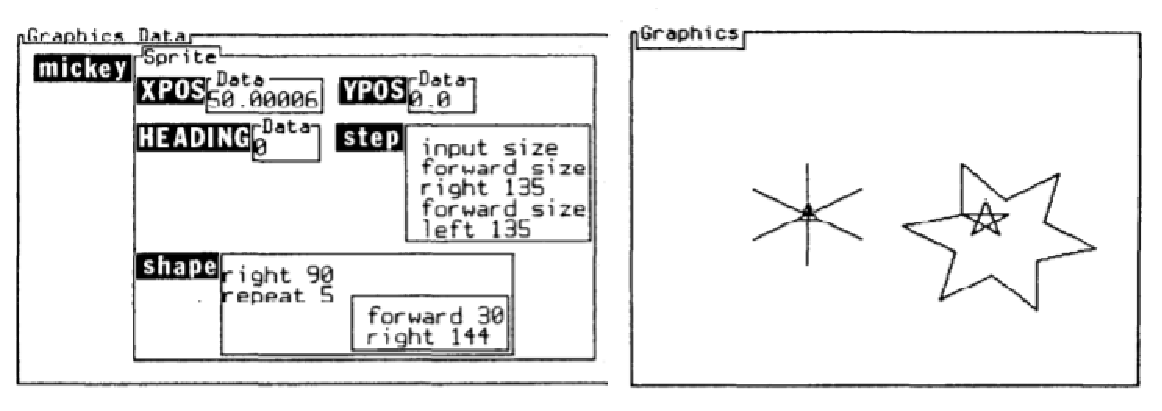
\includegraphics[scale=0.75]{images/CH2BOXER.pdf}
\caption{Graphical user interface for BOXER showing the graphics data (e.g., $x$-position, $y$-position, step instructions) and the resulting graphic for a sprite named mickey.}\label{CH2:BOXER}
\end{figure}

Alternatively, another implementation of computational physics takes the name VPython: the Python programming language with the Visual module.  Historically, the ultimate goal of developing VPython was to ``make it feasible for novice programmers in a physics course to do computer modeling with 3-dimensional visualizations \cite{Sherer2000}.''

Although VPython was ideal for novice programmers, it also catered to more advanced users.  Its basic algorithm is an Euler-Cromer style integration to calculate the contstantly updating position and momentum (or velocity) of an object within a while loop that depends on time.  For example, Fig.~\ref{CH2:MWP} shows the basic structure of a very simple but powerful MWP.  This Euler-Cromer algorithm can be used to analyze very simple situations (e.g., free-fall motion) as well as more complicated and realistic (e.g., the motion of satellites and rockets).

\begin{figure}\center
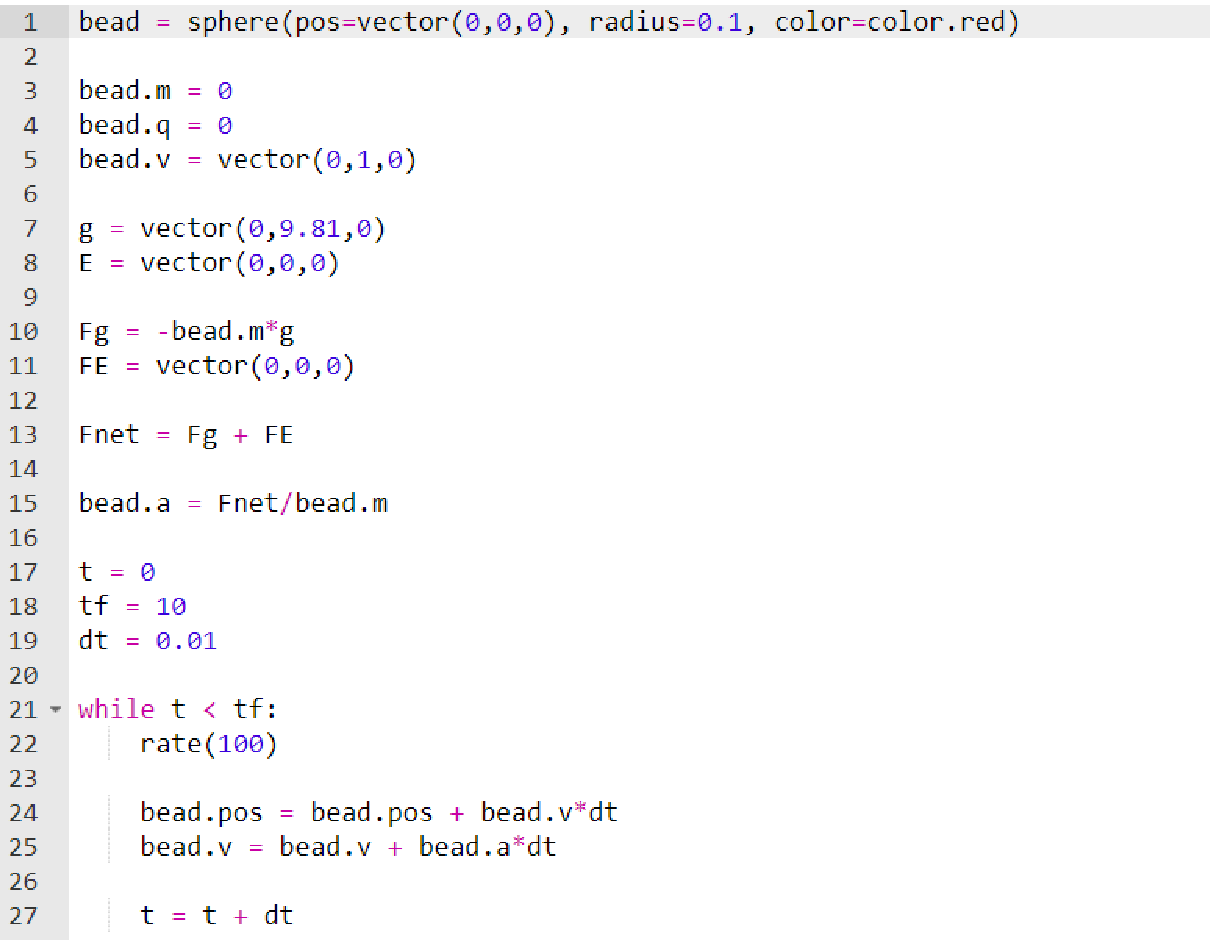
\includegraphics[scale=0.60]{images/CH2MWP.pdf}
\caption{A MWP illustrating that the basic control structure (while loop) and integration algorithm are pre-written so that students can focus on the computational force model that must be constructed in line 11.}\label{CH2:MWP}
\end{figure}

Along with the development of VPython, a software called Easy Java Simulations (EJS) was increasing in use \cite{Esquembre2005}.  These simulations were meant to give students a little more control behind the scenes, like VPython, while still limiting the generalizability like PhET simulations (described below).

For example, a simulation of a pendulum could be constructed in EJS by dragging a particular object (e.g, a pendulum bob) into the model and using their built-in editor to solve the associated differential equation (see Fig.~\ref{CH2:EJS}).  Only a small amount of modification is needed, reducing the load on novice programmers.  This reduction in load through scaffolded programs is very similar to the MWPs used in a lot of the research within PER \cite{Weatherford2011}.

\begin{figure}\center
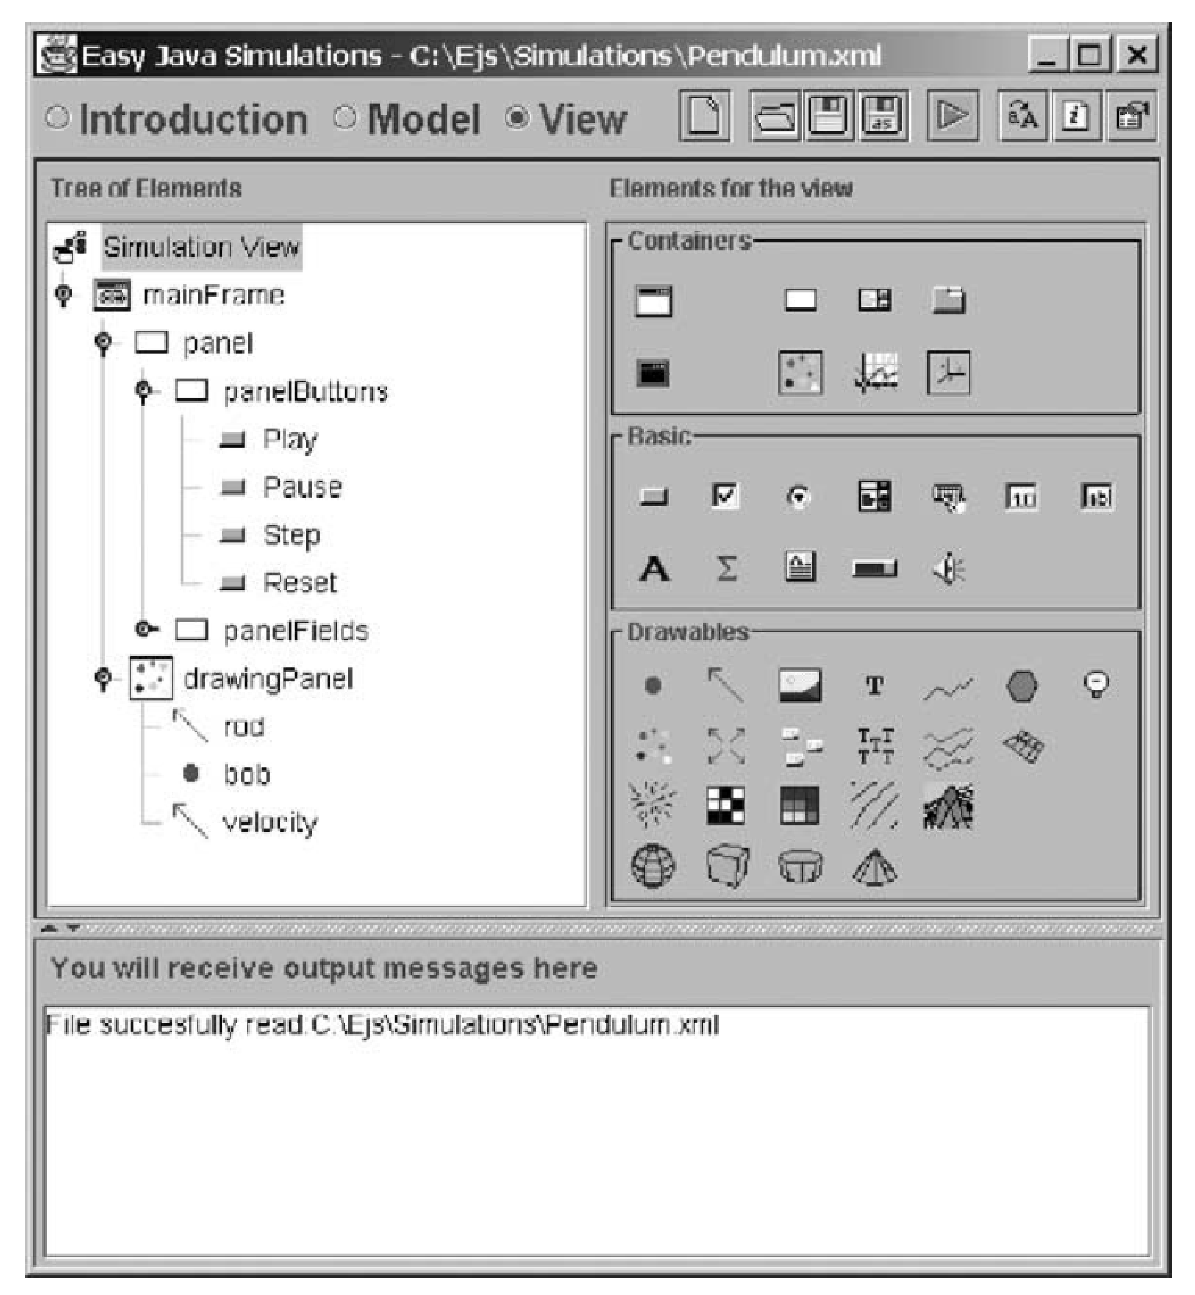
\includegraphics[scale=0.40]{images/CH2EJS.pdf}
\caption{Graphical user interface for an EJS illustrating the ``drag-and-drop'' nature of the software.  Elements (e.g., a pendulum bob) can be added or remove from the different panels (e.g., the drawing panel) in the simulation view.}\label{CH2:EJS}
\end{figure}

Another implementation of computation, frequently used today, are the Physics Education Technology (PhET) simulations \cite{Perkins2006}.  These simulations have realistic graphics that display buttons, sliders, and knobs that can be graphically tweaked to change parameters in a system.  This type of testing -- searching for the effect on a physical system with the variation in a parameter -- is meant to be more engaging and conducive to learning.

For example, the PhET simulation shown in Fig.~\ref{CH2:PhET} is meant to demonstrate the dependence of a pendulum's motion (e.g., its period or amplitude of oscillation) on the various parameters of the system (e.g., the length of the pendulum or the magnitude of friction).  Being able to hold one parameter constant while varying the other helps students to confidently identify its qualitative effect.

\begin{figure}\center
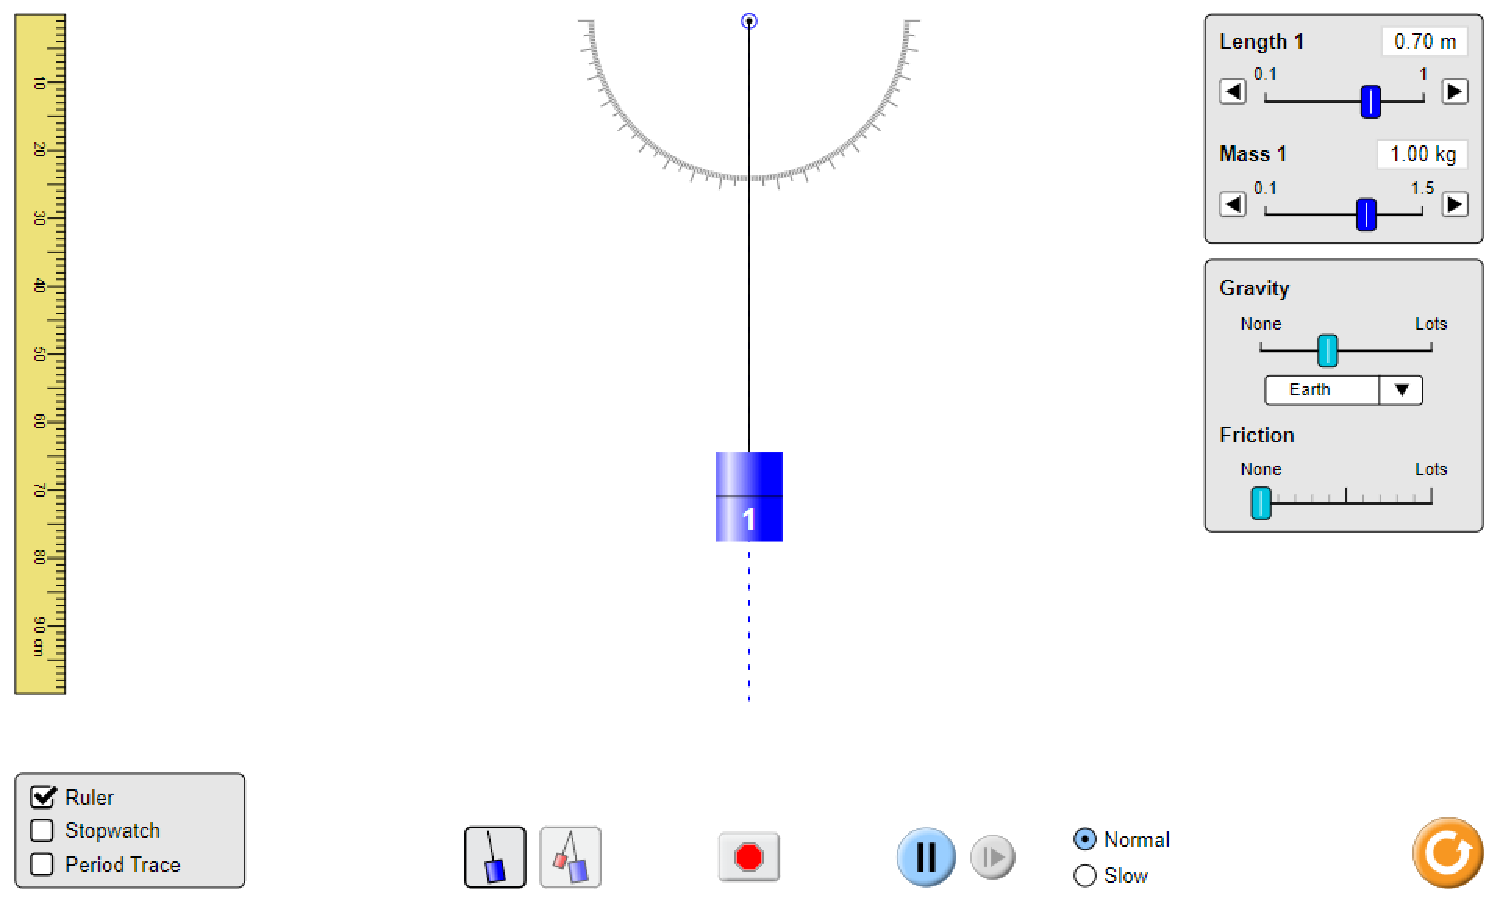
\includegraphics[scale=0.50]{images/CH2PhET.pdf}
\caption{A PhET simulation illustrating the dependence of pendulum motion on the length of the pendulum, the mass of the pendulum bob, the magnitude of the local acceleration due to the gravity, and any frictional forces.}\label{CH2:PhET}
\end{figure}

Finally, one of the more recent implementations of computation at the introductory level is called Glowscript \cite{Chabay2008}.  Glowscript is a variant of VPython which is designed, in part, to easily generate three-dimensional visualizations.  For example, the rather complicated Glowscript program shown in Fig.~\ref{CH2:Glowscript} uses an inverse-square electric field model with for and if loops to generate a visual representation of the electric vector field at any point in space surrounding a discrete charge distribution. 

\begin{figure}\center
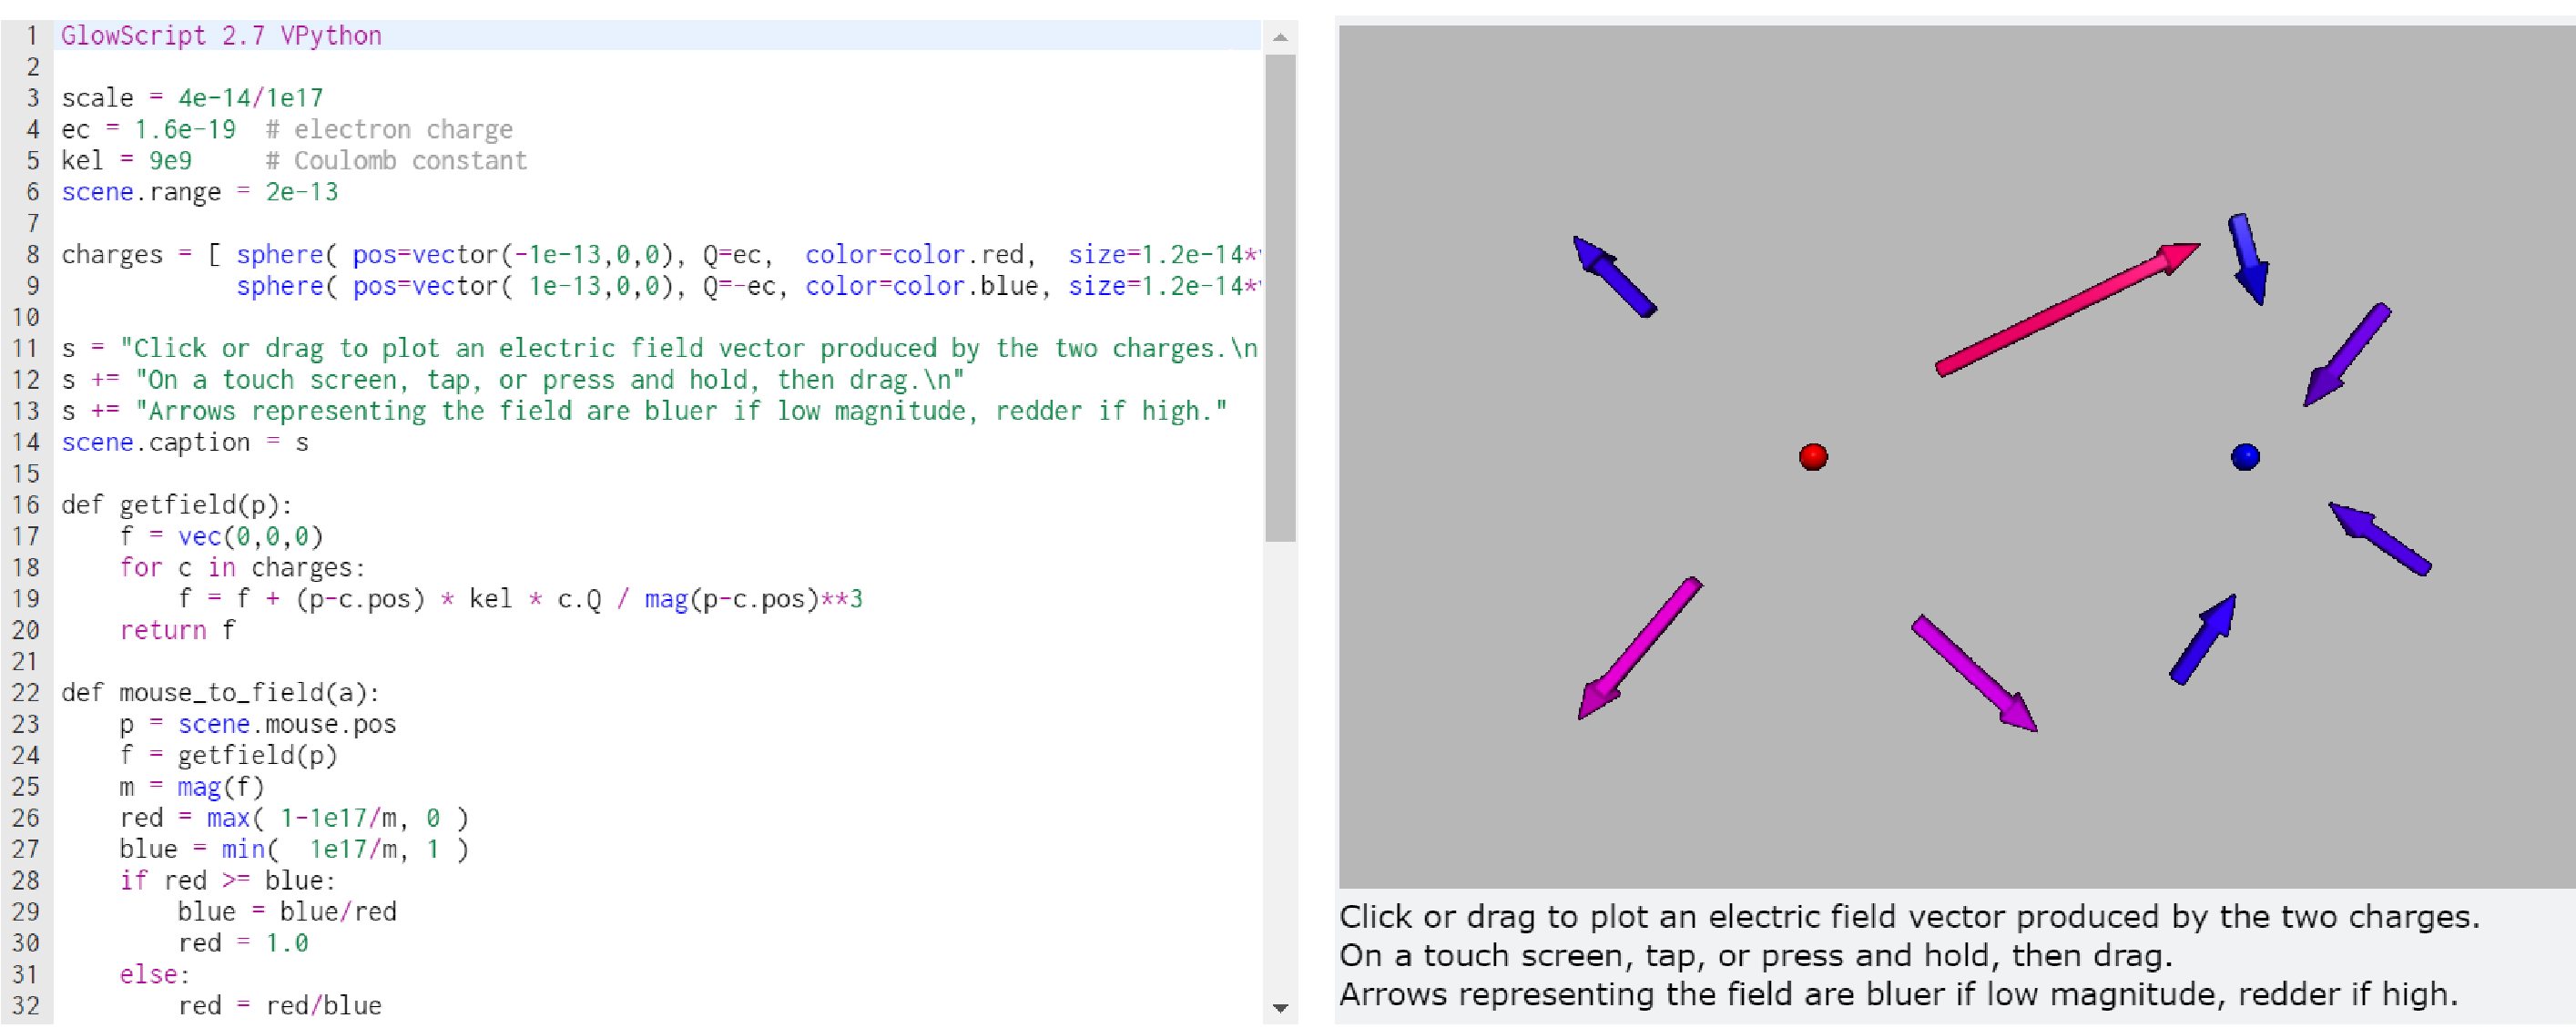
\includegraphics[scale=0.35]{images/CH2Glowscript.pdf}
\caption{Glowscript output demonstrating its ability to generate three-dimensional visualizations of objects, vectors, and graphs.  The ability to quickly and accurately generate three-dimensional vectors allows for more flexibility and a deeper understanding of, for example, electric (vector) fields.}\label{CH2:Glowscript}
\end{figure}

This more realistic and descriptive three-dimensional visualization leveraged by Glowscript and VPython is thought to encourage students to form a deeper understanding of the underlying physics concepts.  Although many different implementations of computation exist \cite{Papert1972,DiSessa1986,Perkins2006,Chabay2008}, research focusing on improving those implementations in PER is still lacking.  Some of the critical results, though, are described below.

\subsection{Results}

In the early 2000s, Chabay began to research the integration of computation into the introductory calculus-based physics course using VPython \cite{Chabay2008}.  This course included a computational curriculum following that presented by \textit{Matter and Interactions}.  Primarily, the courses studied by Chabay focused on the application of the integral equation governing the linear motion of objects (i.e., $d\vec{p}=\vec{F}_{\rm net}\,dt+\vec{p}_{i}$ and $d\vec{r}=\vec{p}/m\,dt$).  These equations were applied iteratively through an Euler-Cromer style integration algorithm, and allowed a more thoroughly analysis of position-dependent forces (e.g., the Newtonian gravitational and spring forces).

Chabay found that one of the positive aspects of including computation at the introductory level was to stimulate creativity in students \cite{Chabay2008}.  This creativity in approaching problem solving is thought to lead students to the construction of more realistic computational models.  In other words, computation allows students to easily verify and/or modify a model, encouraging creativity and a ``guess and check'' approach to problem solving.

She also found that requiring students to program at the introductory physics level was a difficult barrier to overcome.  Given that there is so much content to be covered in so little time in most introductory physics courses, finding the room/time to discuss the basics of programming is difficult.  One of the ways in which this difficulty is overcome is by providing Minimally Working Programs (MWPs) to students.  The MWP for a particular problem usually runs without error from the start (pre-written code), and requires small (or at least localized) changes to the underlying computational models.  For example, see the MWP in Fig.~\ref{CH2:Caballero}.

Around that same time, Kohlmyer dug a little deeper into student performance \cite{Kohlmyer2005}.  He found that, among other things, computational modeling students struggled to recognize that computers could even be used to solve physics problems.  Furthermore, once they did decide to use a computer, they struggled with the concepts and components of creating a computational model.  These results were generated from two experiments: looking at how students approach novel problems with computation and looking at the differences in the fundamental principles used as compared to traditional (i.e., non-computation focused curriculum) students.

Interestingly, he found that students decided to take advantage of the Euler-Cromer style integration in discrete form even when they weren't using a computational model.  That is, students made use of the key conceptual tool that they were taught -- even if just on paper.

He also found that the complex procedure needed to model attractive position-dependent forces was a difficult challenge for students.  Reducing this and other difficulties can be achieved through increasing the frequency of computation throughout the course and requiring computational homework problems.  Kohlmyer made explicit the wide variety of unanswered questions that could be pursued in further research, hinting that the process of ``making assumptions'' and incorporating them into a computational model would be of particular interest.

In 2011, Weatherford began to look at integrating computation into the physics lab curriculum and the sense-making that students engage in \cite{Weatherford2011}.  His study was an in-depth qualitative analysis of group problem solving, focusing on three different contexts: a scattering problem, a spring-mass problem, and a spacecraft-Earth problem.  A coding scheme was developed to help categorize different portions of transcript, as shown in Fig.~\ref{CH2:Weatherford}.

\begin{figure}\center
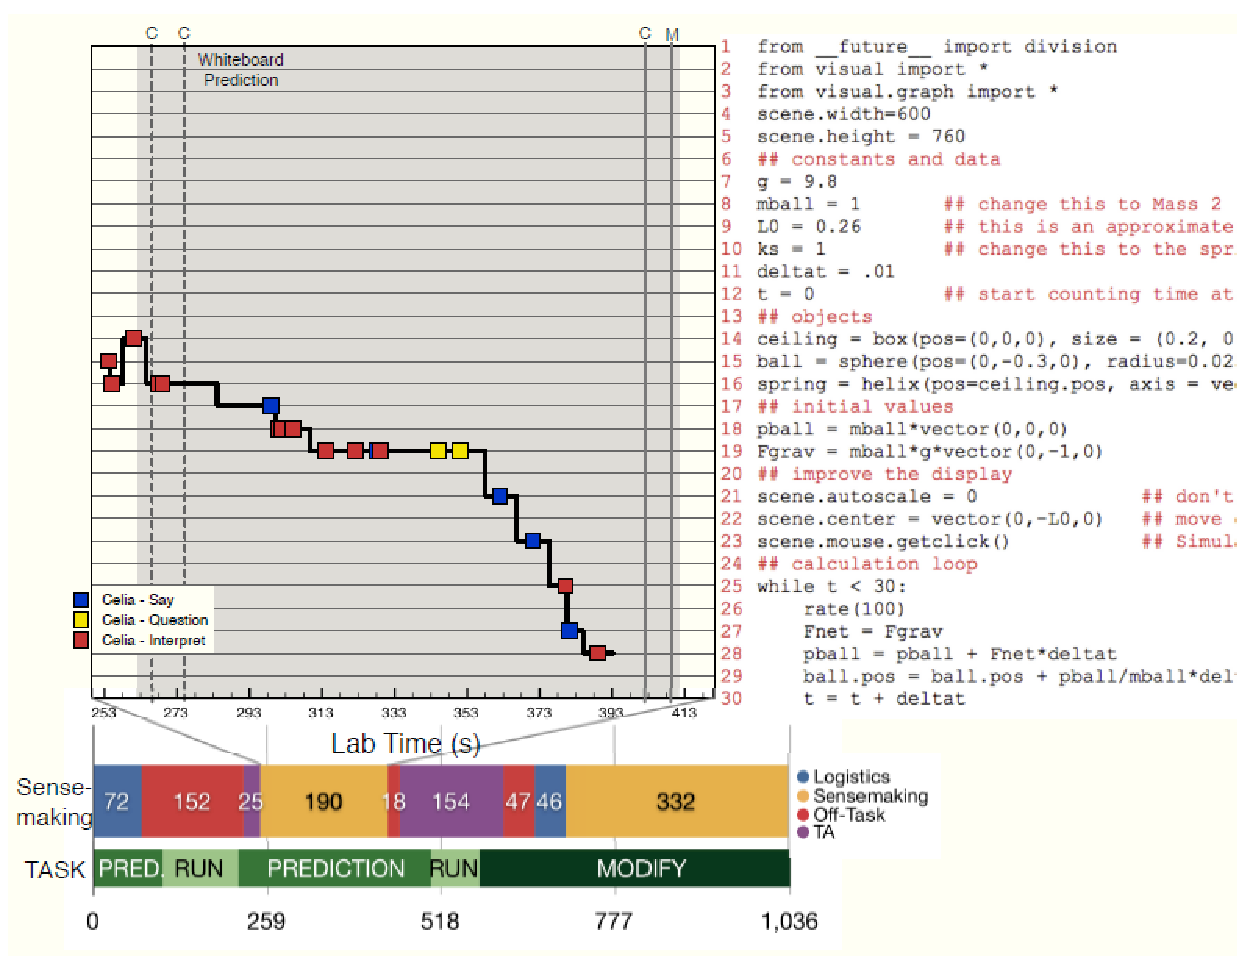
\includegraphics[scale=0.60]{images/CH2Weatherford.pdf}
\caption{A sample of the in-depth analysis Weatherford performed.  Each particular line of code that the group is focusing on is tracked in time and coded according to a scheme.}\label{CH2:Weatherford}
\end{figure}

He found, among other things, that computational physics students were able to reasonably interpret physical quantities according to their variable name.  For example, the mass of a satellite might be defined as \texttt{m.satellite = 1}, or the net force acting on object may be defined as \texttt{Fnet = vector(0,-m*g,0)}.  These pre-written variables are named so as to suggest to the students what physical quantity they represent.  However, the more complicated the definitions get (e.g., a function of multiple variables like \texttt{Fnet = -k * (ball.pos - origin.pos) / mag(L)}, the more students struggled at recognizing it.

Additionally, Weatherford was able to encourage students to begin to incorporate a computational model in a MWP by providing a minimum level of support.  That is, only omitting the fundamental physics calculations that students are meant to engage with (e.g., various computational force models) helps to keep students focused on the physics.  Other tasks that are not physical in nature have a tendency to derail the physics discussion and the problem solving process in general.  For example, ensuring that the end of a spring is connected to the end of a mass in a computational spring-mass analysis begins to overshadow the more fundamental task of incorporating/constructing a position-dependent Hookian spring force.  Alternatively, figuring out how to use the \texttt{mag()} function in Python can sidetrack the ultimate goal of constructing a position dependent gravitational force.

Weatherford clearly pointed out that the MWP activities in their study had much room for improvement, and that more research was needed on fostering student proficiency in computational physics.  The sequence of MWPs in his study didn't quite raise 
students' program comprehension and program interpretation skills to a certain profficiency, but he believes that more research will shed light on the subject.

In 2011, Caballero was able to identify a number of frequent student mistakes which were grouped into three different categories: initial condition mistakes, force calculation mistakes, and second law mistakes \cite{Caballero2011}.  An initial condition mistake might take the form of an incorrect initial velocity or momentum of the satellite.  A force calculation mistake might manifest in a constant spring force rather than a position dependent spring force.  A second law mistake might involve missing the division of the mass from the net force on an object so that the velocity is correctly updated according to the acceleration.  These frequent mistakes result in both unexpected and physically inaccurate visualizations.

Based on his analysis of the satellite-Earth problem, shown in Fig.~\ref{CH2:Caballero}, he concluded that the majority of students ($\sim\SI{60}{\percent}$) were able to correctly computational model novel physics problems and that the practice of debugging would serve students well.  Particularly, the act of troubleshooting syntax errors as well as the act of troubleshooting of \textit{physics} errors.

\begin{figure}\center
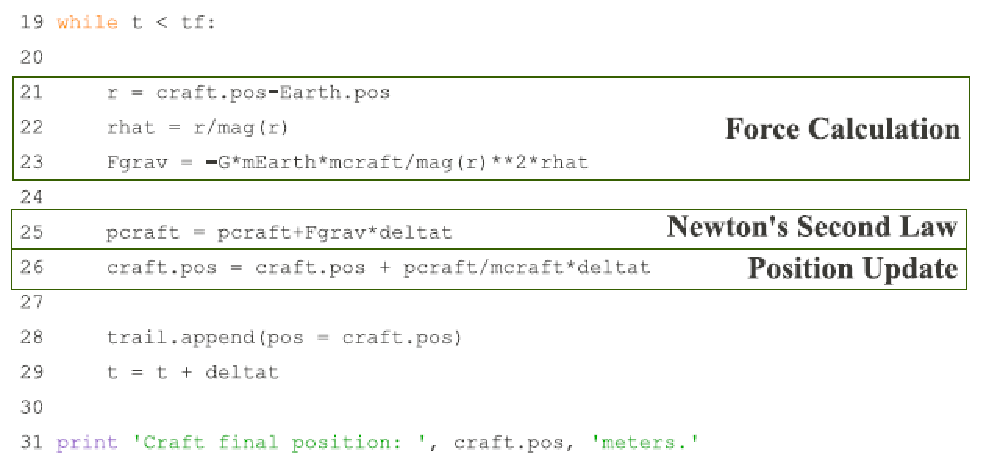
\includegraphics[scale=0.8]{images/CH2Caballero.pdf}
\caption{An expected solution to a computational satellite-Earth problem where the Newtonian gravitational force has been constructed from a separation vector and its magnitude.  The force calculation has been incorporated into the momentum through Newton's second law, and the momentum is incorporated into the position through a position update.}\label{CH2:Caballero}
\end{figure}

\subsection{Remaining questions}

Although many aspects of computation and computational thinking at the introductory level have been studied, there are still many unanswered questions within physics education.  Particularly, as to the types of practices students are engaging in that are indicative of computational thinking.  More research is needed to not only more clearly define the computational practices observed in introductory physics, but also to more clearly understand the habits of mind and types of thinking that students are engaging in.

Add some.

\section{Framework}

Recently, a framework for identifying the computational practices that are indicative of computational thinking has been proposed by Weintrop et. al.  This framework was developed using existing literature on computational thinking, interview with mathematicians and scientists, and most importantly, computational activities from general science and mathematics classrooms.

In order to develop their framework, a literature review was performed to generate an intial set of $10$ math and science practices.  These initial practices are repeatedly cited as being central to computational thinking.  For example, the broad and repeatedly cited practice of generating algorithmic solutions might require a student to engage with a differential equation algorithm.  These broad initial practices were used to guide the subsequent qualitative analysis.

Using the initial practices resulting from the literature review, two reviewers independently coded for the various ``facets'' of computational thinking that were required by the curricular materials.  They analyzed $32$ different computational activities from chemistry to programming, resulting in $208$ facets which were grouped into $45$ different practices.

Next, a review process incorporating feedback from multiple sources (e.g., teachers, content experts, and curriculum designers) was used to reduce the $45$ practices into $27$, which were further organized into $5$ different categories.  Further, external interviews were conducted with $16$ K-12 science and mathematics teachers, helping to reduce the $27$ practices into $22$ fitting $4$ different categories, shown in Tab.~\ref{CH2:Framework}.

\begin{table}[hb]\centering
\begin{tabular}{llll}\hline\hline
Data         & Modeling     & Solving     & Systems       \\\hline
Creating     & Conepts      & Preparing   & Investigating \\
Collecting   & Testing      & Programming & Understanding \\
Manipulating & Assessing    & Choosing    & Thinking      \\
             &              & Creating    & Communicating \\
             &              & Debugging   & Defining      \\\hline\hline
\end{tabular}
\caption{The framework developed by Weintrop et. al to describe the computational practices observed in science and mathematics classrooms.  Each category contains between five and seven individual practices, and each practice has between two and seven fundamental characteristics.}\label{CH2:Framework}
\end{table}

Finally, $15$ interviews with STEM professionals were conducted to rate their framework according to its appicability to authentic professional practices and to give direction for future improvement.  For example, interviews showed that the practice of testing and debugging was a crucial practice that was not adequately captured by the framework -- an improvement that should be made on future iterations of the framework.

The four different categories of practices are labeled as data, modeling and simulation, computational problem solving, and systems thinking practices.  The data practices focus mostly on the creation and visualization of data.  The modeling and simulation practices focus mostly on the design, construction, and assessment of a computational model.  The problem solving practices focus mostly on programming and debugging, while the systems thinking practices are a little more abstract and focus mostly on the structure of the program itself.

As a more concrete example, the computational practice of creating data (a data practice) has three fundamental characteristics: the creation of a set of data, an articulation of the underlying algorithm, and a use of the data to advance their understanding of a concept.  The more of the characteristics that we observe in a particular excerpt, the more confident we are that that excerpt can be classified as that practice.

Although each practice is defined like this, according to Weintrop et. al, the characteristics themselves are rather vague (similar to the operational defintions from the NGSS).  For example, the computational practice of assessing computational models requires the identification of a phenomenon, a computational model, and a comparison made between the two.  Although it is clear what a comparison would look like in any situation, the phenomena studied and the models used will depend greatly on the context (See Ch.~\ref{CH3:Context}).  For this reason, much more work must be done to clearly define computational thinking within introductory physics classrooms -- a central task to this thesis.

Ultimately, Weintrop found three main benefits to including computation: it builds on the reciprocal relationship between computationl thinking and STEM domains, it engages learners as well as instructors, and it introduces an authentic and modern element of doing science.  However, he is clear to indicate that more research is needed to better address the challenge of educating a technologically and scientifically savvy population.  This thesis attempts to improve that education process by providing clear and precise defintions of the computational practices that are indicative of computational thinking.

\section{Task analysis}

In order to give this research a solid foundation, early on, we conducted a task analysis of a complicated computational physics problem.  A task analysis consists of breaking a problem down into multiple smaller but manageable sub-tasks.  These sub-tasks can then be searched for within data.  For example, an expert group might proceed in predicting the motion of an object by first constructing an Euler-Cromer style algorithm, constructing the various forces, and then construct the initial parameters of the system.

This type of process was used by Catrambone to show that breaking a problem down into smaller but manageable sub-tasks helps students to transfer knowledge to new and novel problems \cite{Catrambone1998}.  He and others believe that it is a heriarchical structure of tasks rather than a linear structure of tasks that students need to transfer knowledge to new and novel situations.  The flexibility of a heirarchical structure is thought to support a more varied approach to solving a problem.

They performed three experiments, each focusing on how students transfer knowledge to new and novel problems.  The first experiment was a comparison between the meaningfulness of a label's name.  They found that the more meaningful the label was, the better prepared students were to solve new and novel problems.  The second was a deeper study of the connections between labels and sub-tasks.  They found, to a reasonable degree, that there was a fundamental connection between labels, sub-tasks, and how they were grouped.  The third was a talk-aloud study that looked at self-explanation while solving problems.  They found that aptly named labels could be used to cue students to group sub-tasks and explain their purpose through self-explanation.

The task analysis of the problem that this thesis focuses on was initially constructed by a single content expert.  After the first iteration it was presented to additional experts.  Through the discussions surrounding these iterations, it became clear that the construction of the position dependent Newtonian gravitational force in code is a multi-step procedure involving a number of different sub-tasks.  The task analysis was iteratively refined through this process until all experts agreed that the sub-tasks shown in Tab.~\ref{CH3:TaskAnalysis} were sufficiently described/defined to be useful in video analysis.

\begin{table}[hb]\centering
\begin{tabular}{lr}\hline\hline
Step (Sub-Task) & Associated Code \\\hline
Construct separation vector & \begin{lstlisting}
sep = obj2.pos
\end{lstlisting}\\
between interacting objects & \begin{lstlisting}
         - obj1.pos
\end{lstlisting}\\\hline
Construct the unit vector & \begin{lstlisting}
usep = sep/mag(sep)
\end{lstlisting}\\\hline
Construct the net force & \begin{lstlisting}
Fnet = -G*m1*m2*usep
\end{lstlisting}\\
vector & \begin{lstlisting}
         /mag(sep)**2
\end{lstlisting}\\\hline
Integrate the net force over & \begin{lstlisting}
obj.p = obj.p + Fnet*dt
\end{lstlisting}\\
time into momentum & \\\hline\hline
\end{tabular}\caption{Some of the necessary steps that must be taken when constructing a Newtonian gravitational force in code.  Each step is associated with the construction/modification of a line of code.\label{CH3:TaskAnalysis}}
\end{table}
 
On top of this expert generated solution, there are many other (both expected and unexpected) student generated solutions that we observe in the data.  However, the expert generated solution is an ideal path to follow and so the instructors try to keep groups moving in this direction.  For example, a sufficient force model be constructed in terms of the polar and azimuthal angle of the satellite, although it requires a substantial amount of work to code.  Both the expert and student generated solutions are a good place to look for evidence of computational thinking and its accompanying practices.

\section{Thematic analysis}

The qualitative methodology that we used follows a widely used method within psychology: thematic analysis.  However frequently used, thematic analysis is rarely defined.  Accordingly, Braun et. al has provided clear guidelines for conducting a scientifically reliable and valid qualitative analysis \cite{Braun2008}.

According to Braun, a thematic analysis is a ``method for identifying, analyzing, and reporting patterns (themes) within data.''  This method consists of $6$ different phases, usually followed linearly, to finally produce a report (i.e, a thematic map) of the various themes and their relationships within a set of qualitative data.

The first phase focuses on transcribing and farmiliarizing yourself with the data.  Reading through the transcripts multiple times helps to generate preliminary ideas that can be coded for further investigation.  Next, each code must be collated with the corresponding transcript so as to provide a context.  After the codes have been collated with the corresponding transcript, themes begin to emerge in the third phase.

Reviewing any themes that emerge, particularly against the coded extracts and the transcript as a whole, leads to the next phase of defining, validating, and naming any themes.  These themes can finally be presented in a scholarly report with step-by-step transcript analysis and/or a thematic map.  A thematic map, shown in Fig.~\ref{CH2:Map}, shows not only the components of a theme, but also the \textit{relationships} between those components.

\begin{figure}\center
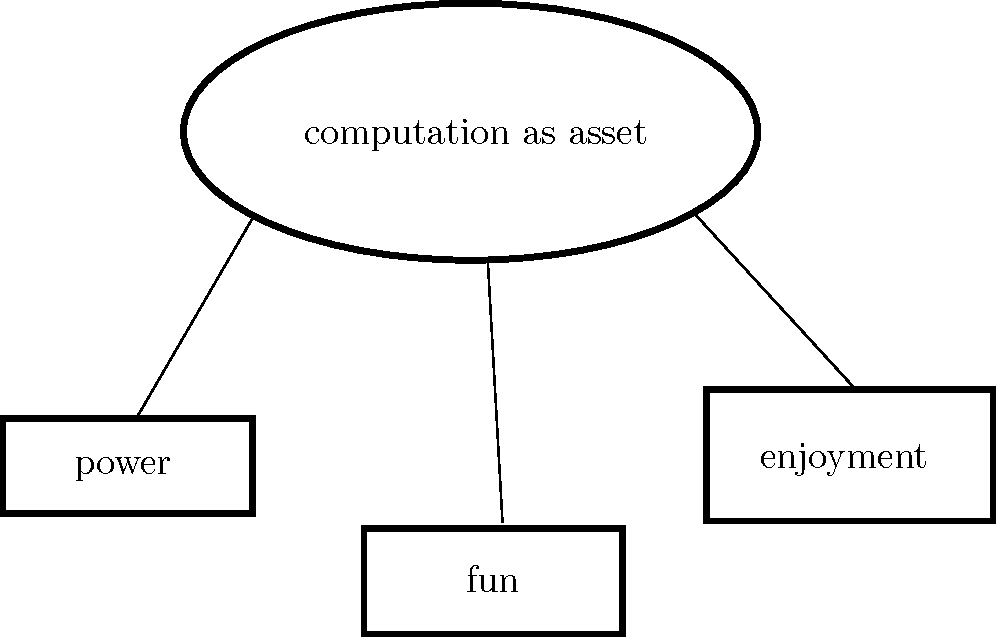
\includegraphics[scale=0.60]{images/CH2Map.pdf}
\caption{A final thematic map showing the components of a theme named ``computation as asset.''  The main components of this theme are ``power,'' ``fun'', and ``enjoyable.''}\label{CH2:Map}
\end{figure}

Braun is clear to point out that there are many pitfalls associate with thematic analysis, and that researchers must be cognizant of them through every phase of the process.  For example, one of the pitfalls she highlights is a possible mismatch between the data and the analytic claims that are being made.  In other words, it is important to always closely tie your claims with the actual data.  This closeness of the claims to the data can be ensured through frequent inter-rater reliability checks.

Given the flexibility of qualitative anlysis, it is important to be clear and explicit about the decisions being made throughout the entire process.  Braun has presented $15$ criteria for conducting a good qualitative thematic analysis.  These criteria focus on things like checking that each data item has been given equal attention, and checking that themes are internally coherent, consistent, and distinctive.

%
%	CONTEXT (P3)
%

\chapter{Context}\label{CH3:Context}

It is important to understand the course from which we have collected our data to better understand the results of our study.  That course -- called Projects and Practices in Physics (${\rm P}^{3}$) -- is based on a social constructivist theory of learning and a flipped/problem-based pedagogy.  In other words, students familiarize themselves with relevant material before coming to class, where they will work in small groups to actively and socially construct knowledge while solving complex analytical and computational physics and engineering problems.  The course has intentionally been designed to encourage computational thinking wherever possible.  Specifically, computational thinking has been incorporated into the notes, pre- and post-class homework, in-class feedback and assessments, and a selection of the in-class problems.

\section{Course design}

Each week in ${\rm P}^{3}$, students are expected to do a number of things. They must complete the pre-class homework which is based on information that they should gather from the pre-class notes.  They must then work in small groups (usually between three and four members) on two related analytical problems or a mixture of one related analytical and one related computational.  These problems are delivered during the two two-hour weekly meetings (See Fig.~\ref{CH3:Schedule}).  For the computational problem, that means reading and interpreting pre-written code (i.e., a minimally working program) while they design, assess, and construct a computational force model.  The small group is facilitated by either a course instructor, graduate teaching assistant, or undergraduate learning assistant who will ask relevant and pertinent follow-up questions.  There are also post-class homework questions based on information gathered from the pre-class notes and the in-class problems that are due at the end of the week.  This all occurs while students simultaneously prepare for the following week.

\section{VPython}

Given that the vast majority of students enter ${\rm P}^{3}$ with little to no prior programming experience, we need to ensure that they are prepared to handle computational problems early in the semester.  One way that we can ensure this is by requiring students to engage with the fundamental programming ideas (e.g., iteration through a while loop control structure or pre-defined mathematical functions) before coming to class through pre-class homework and notes.  These notes and homework questions highlight the fundamental physical and programming ideas specific to VPython and the computational problems that will be delivered in class.

For example, consider the portion of the course notes shown in Fig.~\ref{CH3:VPythonNotes}.  These notes are made available to the students at the beginning of the semester and are meant to provide students with a basic understanding of the utility of VPython along with a list of common errors that novice programmers must frequently deal with.  These notes provide not only a description of the error, but also a procedure for removing it while students are troubleshooting and debugging in-class code.  Troubleshooting and debugging are two of the problem solving practices indicative of computational thinking that we focused our analysis on.

\begin{figure}[ht]\centering
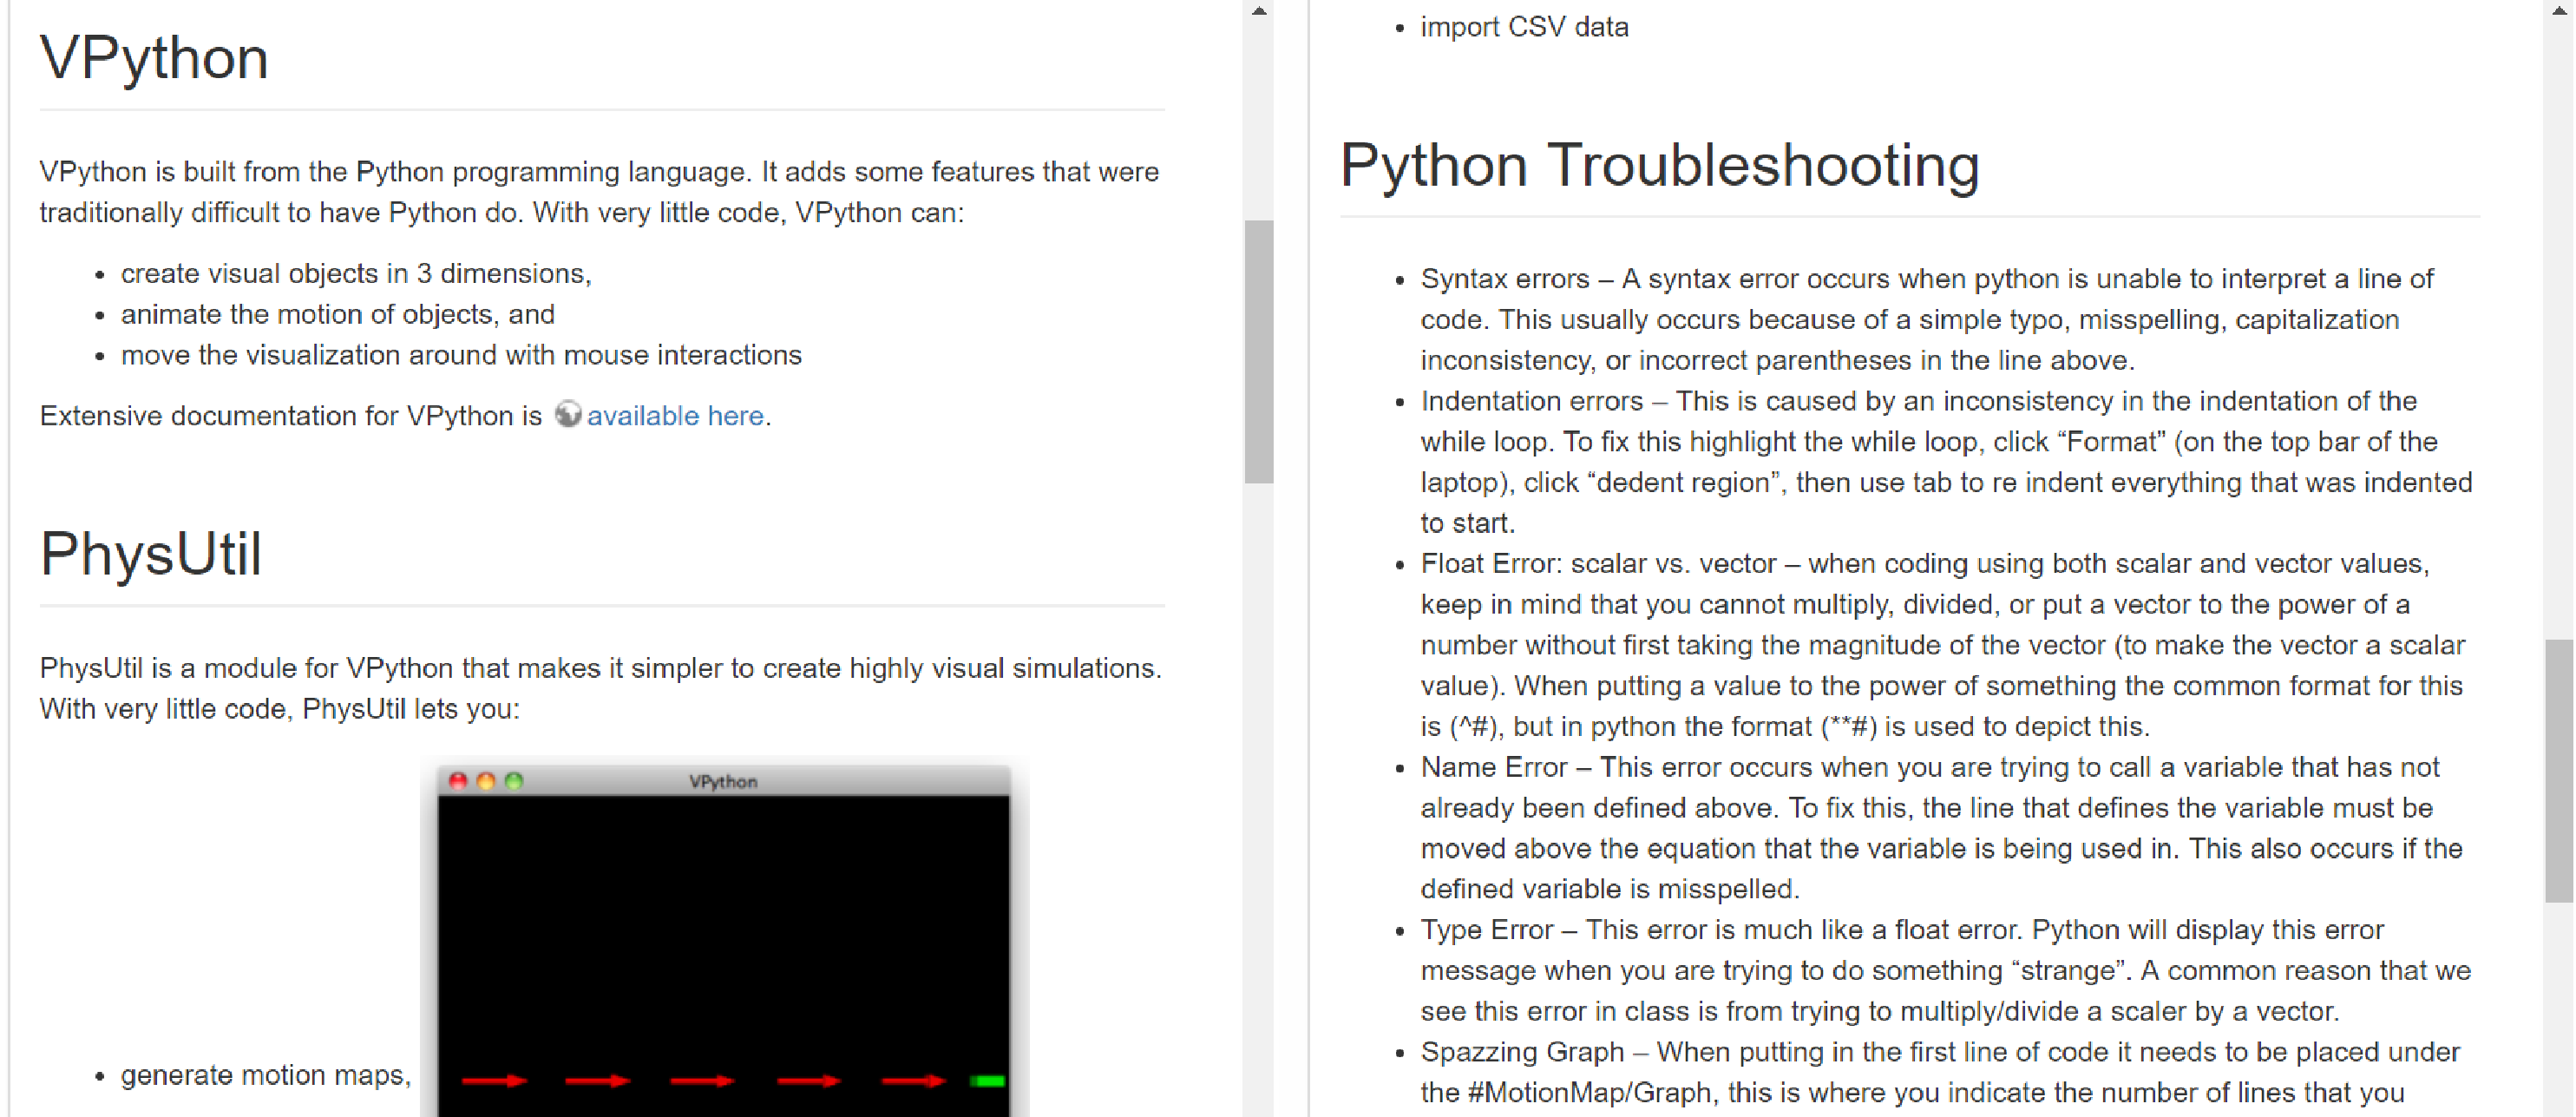
\includegraphics[scale=1]{images/CH3VPythonNotes.pdf}
\caption{Portion of on-line notes that is made available to the students during the first week of the course.  These notes introduce the fundamenatal programming ideas and a list of common errors with tips and tricks.}\label{CH3:VPythonNotes}
\end{figure} 

\section{Pre-class work}

There are other weekly notes, made available to the students at the beginning of every week, focusing more on the fundamental physical ideas that will be used during class.  For example, during the third week the notes focus on uniform circular motion (most heavily used during the week's analytical problem) and the Newtonian gravitational force (most heavily used during the week's computational problem).

Aside from notes, material is also delivered to the students through weekly pre-class homework questions.  Consider the pre-class homework questions shown in Fig.~\ref{CH3:PreClassQuestion} that are made available at the beginning of the third week of the course.  This question is meant to demonstrate that there are multiple correct ways that a unit vector can be constructed in code.  Given the nature of the corresponding week's computational problem (see Sec.~\ref{CH3:SatelliteProblem}), we expect students to be able to draw on and take advantage of this knowledge when faced with a related albeit more complicated problem.  That is, we expect students to be choosing between competing solutions.  Choosing between competing solutions is a problem solving practice indicative of computational thinking that we focused our analysis on.

\begin{figure}[ht]\centering
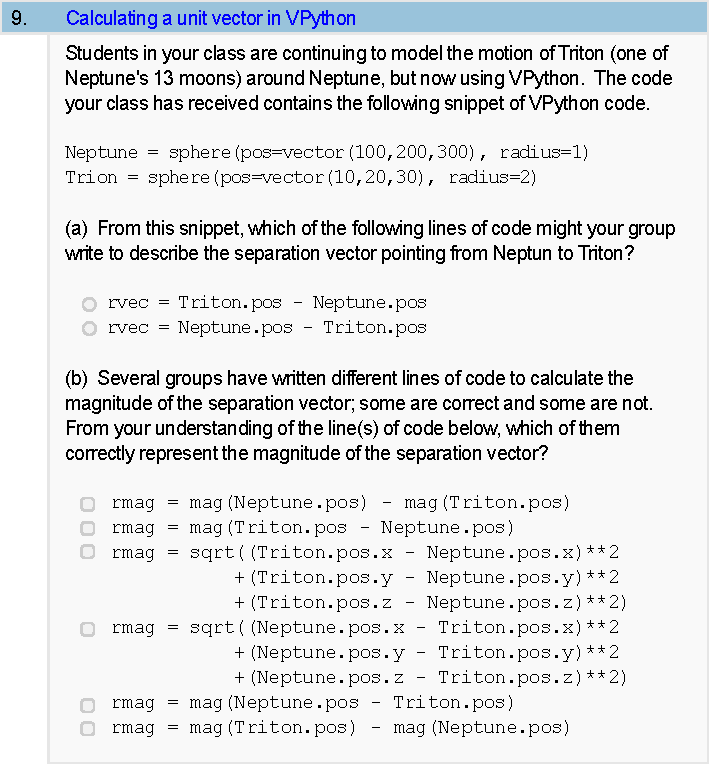
\includegraphics[scale=0.75]{images/CH3PreClassQuestion.pdf}
\caption{Pre-class homework question focusing on the different ways that the magnitude of a vector can be constructed in VPython code: explicitly coding the square root of the sum of the squares of the components and using the pre-defined Python ``magnitude'' function.}\label{CH3:PreClassQuestion}
\end{figure} 

Targeted pre-class homework questions were also developed to help students overcome challenges based on the task analysis.  For example, the pre-class homework questions shown in Fig.~\ref{CH3:PreClassQuestion} were developed to facilitate student understanding of the unit vector of a separation vector between two objects prior to working on the related computational problem.  Given that students must grapple with using a separation vector to construct a unit vector in code during the week, these questions help to place them in the Zone of Proximal Development (ZPD) \cite{Vygotsky1980}.  Constructing computational models is (unsurprisingly) a computational modeling practice indicative of computational thinking that permeates our data.

\section{In-class work}

There are a number of in-class computational problems spread out throughout the semester (see Fig.~\ref{CH3:Schedule}).  The first few computational problems focus on different force models (i.e., no force, a constant force, a non-constant force) and the resulting linear motion of objects.  The last few computational problems focus on extended objects and their rotation.  While solving these problems, groups are expected to engage in a number of computational practices that the problems have been designed around: \begin{enumerate}
\item[P1.] developing and using models,
\item[P2.] planning and carrying out investigations,
\item[P3.] analyzing and interpreting data,
\item[P4.] using mathematics and computational thinking,
\item[P6.] constructing explanations,
\item[P7.] engaging in argument from evidence.
\item[P8.] and obtaining, evaluating, and communicating information.
\end{enumerate}

%\begin{landscape}
%\thispagestyle{empty}
\begin{figure}[ht]\centering
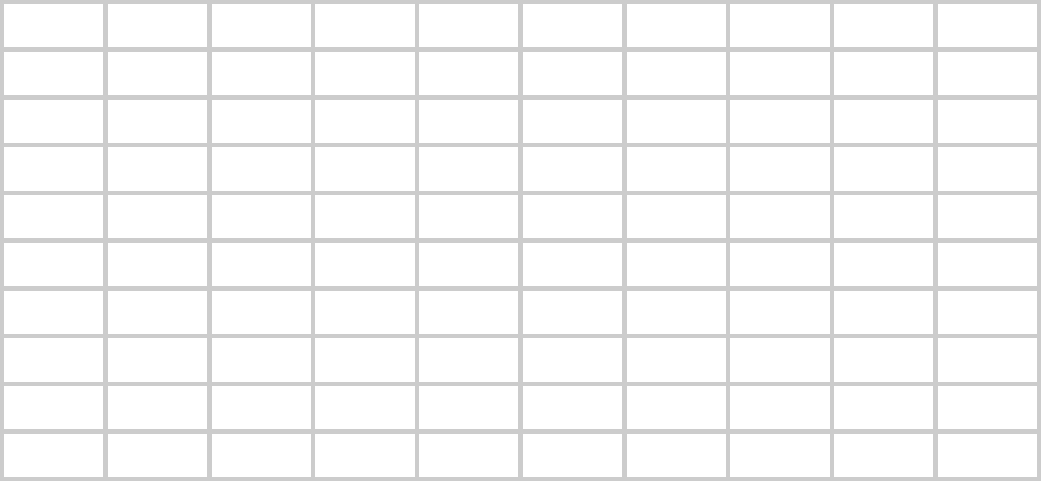
\includegraphics[scale=0.60]{images/CH3Schedule.pdf}
\caption{A schedule for the semester focusing on topics covered, homework/reading deadlines, and in-class problems.  \textbf{Should this figure be on a landscape page?}}\label{CH3:Schedule}
\end{figure}
%\end{landscape}

One of the scientific practices used heavily on both analytic and computation days is that of (P1) developing and using models.  Whether those models be mathematical or computational, we expect students to not only work together in groups to develop the model, but also to utilize that model in further investigations.  This type of scientific practice (P1) and its associated learning goals \cite{Irving2017} were further used to generate the in-class project that this thesis focuses on.

\subsection{Analytic problem}

In the third week of the course, students are asked to analyze the motion of a satellite orbiting Earth both analytically and computationally.  For the analytic day, the groups were asked to solve for the magnitude of the velocity and radius needed by a satellite to be held in a geostationary orbit.  This involves identifying two relevant equations in two unknowns and combining them to solve for the desired radius and magnitude of velocity.  The information gathered during this problem can be used in the following computational problem, and the group facilitators are often observed referencing this information.

\subsection{Computational problem}

This thesis focuses on the third and most complicated computational problem delivered to the students, shown in both Figs.~\ref{CH3:Schedule} and \ref{CH3:SatelliteProblem}. Given its complexity, we developed a framework to help guide and ground our analysis.  This framework was constructed with the help of a task analysis (see Sec.~\ref{CH2:Background}) of the problem.  Ultimately, students must design, construct, and asses a computational model for the Newtonian gravitational force acting on a satellite in geostationary and other more general orbits.

\begin{figure}[ht]\centering
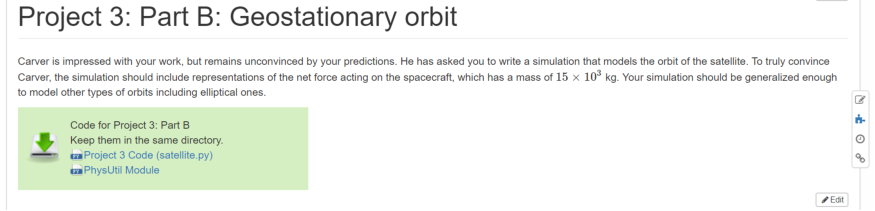
\includegraphics[scale=1]{images/CH3SatelliteProblem.pdf}
\caption{The Newtonian gravitational force problem statement delivered to the students in the third week of class.}\label{CH3:SatelliteProblem}
\end{figure}

Once the correct force has been correctly coded, the group must also grapple with adding in a visualization of a vector representing the force that they have just added.  This type of motion diagram is meant to show that the gravitational force vector resulting in the orbit always points radially inward (toward the Earth).  This task requires students to program as well as allows them to more easily check their conceptual understanding.  Using computational models to understand a concept is a computational modeling and simulation practice that is indicative of computation thinking.

Additionally, in order to check that their model can produce a geostationary orbit, groups are asked to generate a graph showing the magnitude of the separation between the satellite and the center of the Earth vs. time.  This allows them to check for a constant distance which implied a circular orbit.  This task is meant, among other things, to encourage students to visualize data, another computational practice indicative of computational thinking.

\subsubsection{Minimally working programs}

While beginning the problem, the group will observe a Minimally Working Program (MWP) similar to those seen in the two previous computational problems.  This MWP has all of the structure of the code correct (the while/calculation loop and the Euler-Cromer integration) but is missing the computational force acting on the satellite (along with some inaccurate numerical values).  The initial MWP code with its initial visualization are shown in Fig.~\ref{CH3:InitialCodeVisual}.

\begin{figure}[ht]\centering
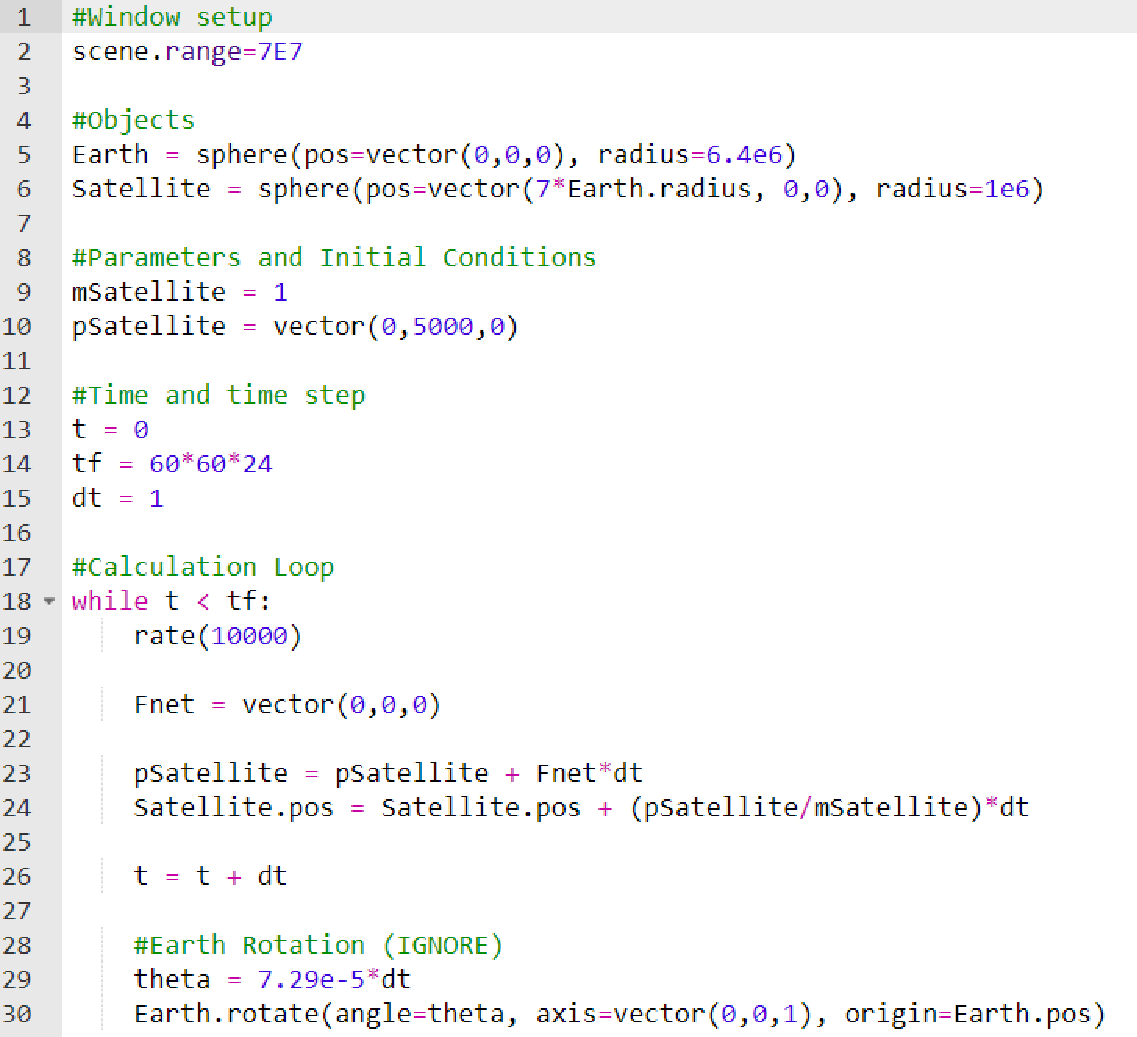
\includegraphics[scale=0.40]{images/CH3InitialCode.pdf}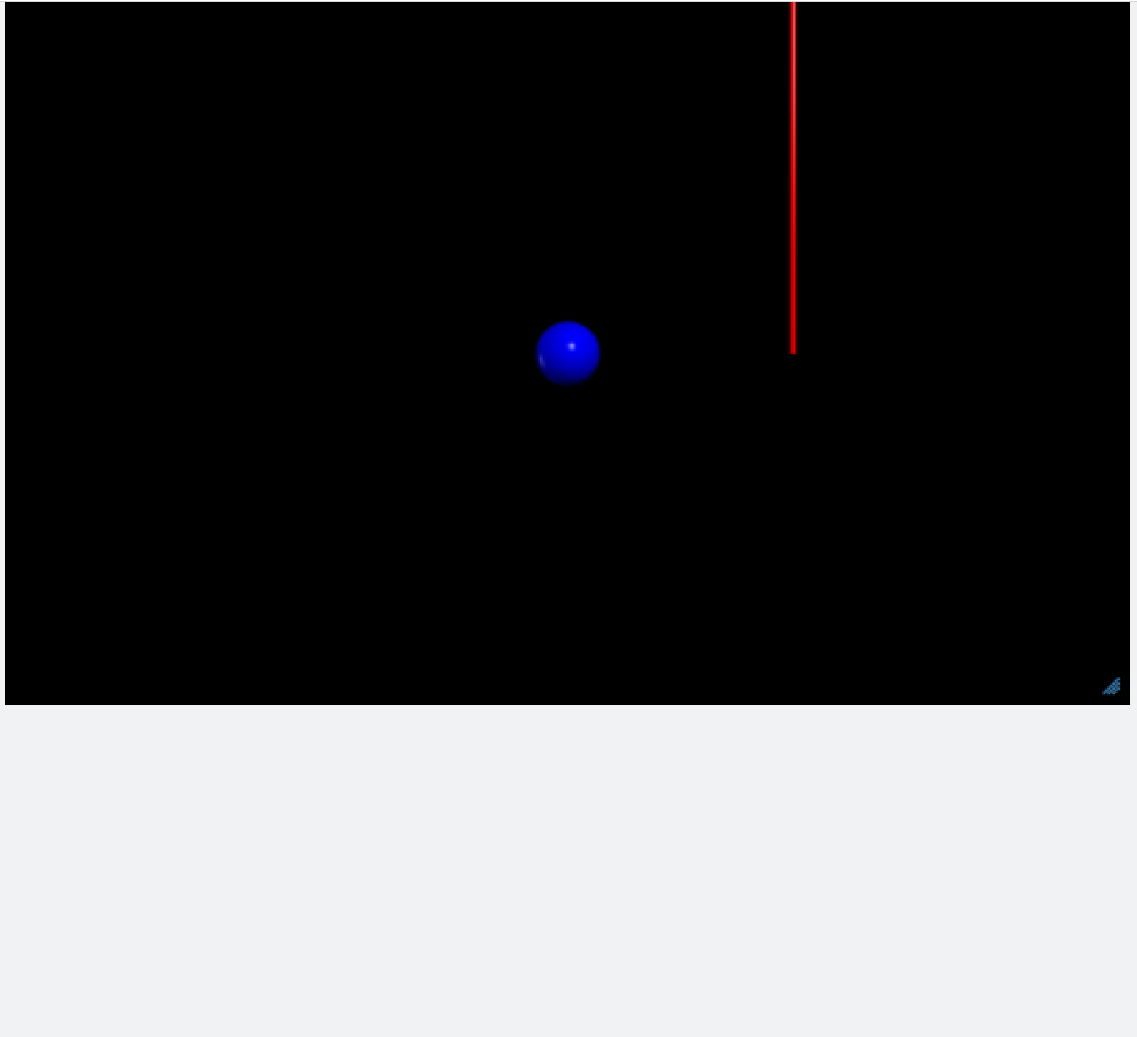
\includegraphics[scale=0.40]{images/CH3InitialVisual.pdf}
\caption{The initial code and visualization of the MWP that is given to the students in the third week of the course.}\label{CH3:InitialCodeVisual}
\end{figure}

Thus, the main task of the group is to construct a physically correct force model in code.  Secondarily, they must modify numerical values to reflect the phenomenon being modeled.  Ideally, this force model will be of a Newtonian gravitational form (i.e., $F_{G}\sim1/r^{2}$) with a direction coded in terms of a separation vector (i.e., $\hat{F}_{G}\sim\vec{r}/r$).  However, there are many other ways to go about this, and we do frequently observe groups working with other models (e.g., a centripetal force).

\subsubsection{Tutor questions}

There are a number of pre-written tutor questions as well as many on-the-fly questions generated by the tutors while in class.  These questions are meant to check the students for conceptual understanding as well as to direct students toward the correct solution.  For example, the tutor questions shown in Fig.~\ref{CH3:TutorQuestion} are meant to ensure that the model the group has constructed is actually general enough to generate all types of elliptical orbits given various initial conditions.

\begin{figure}[ht]\centering
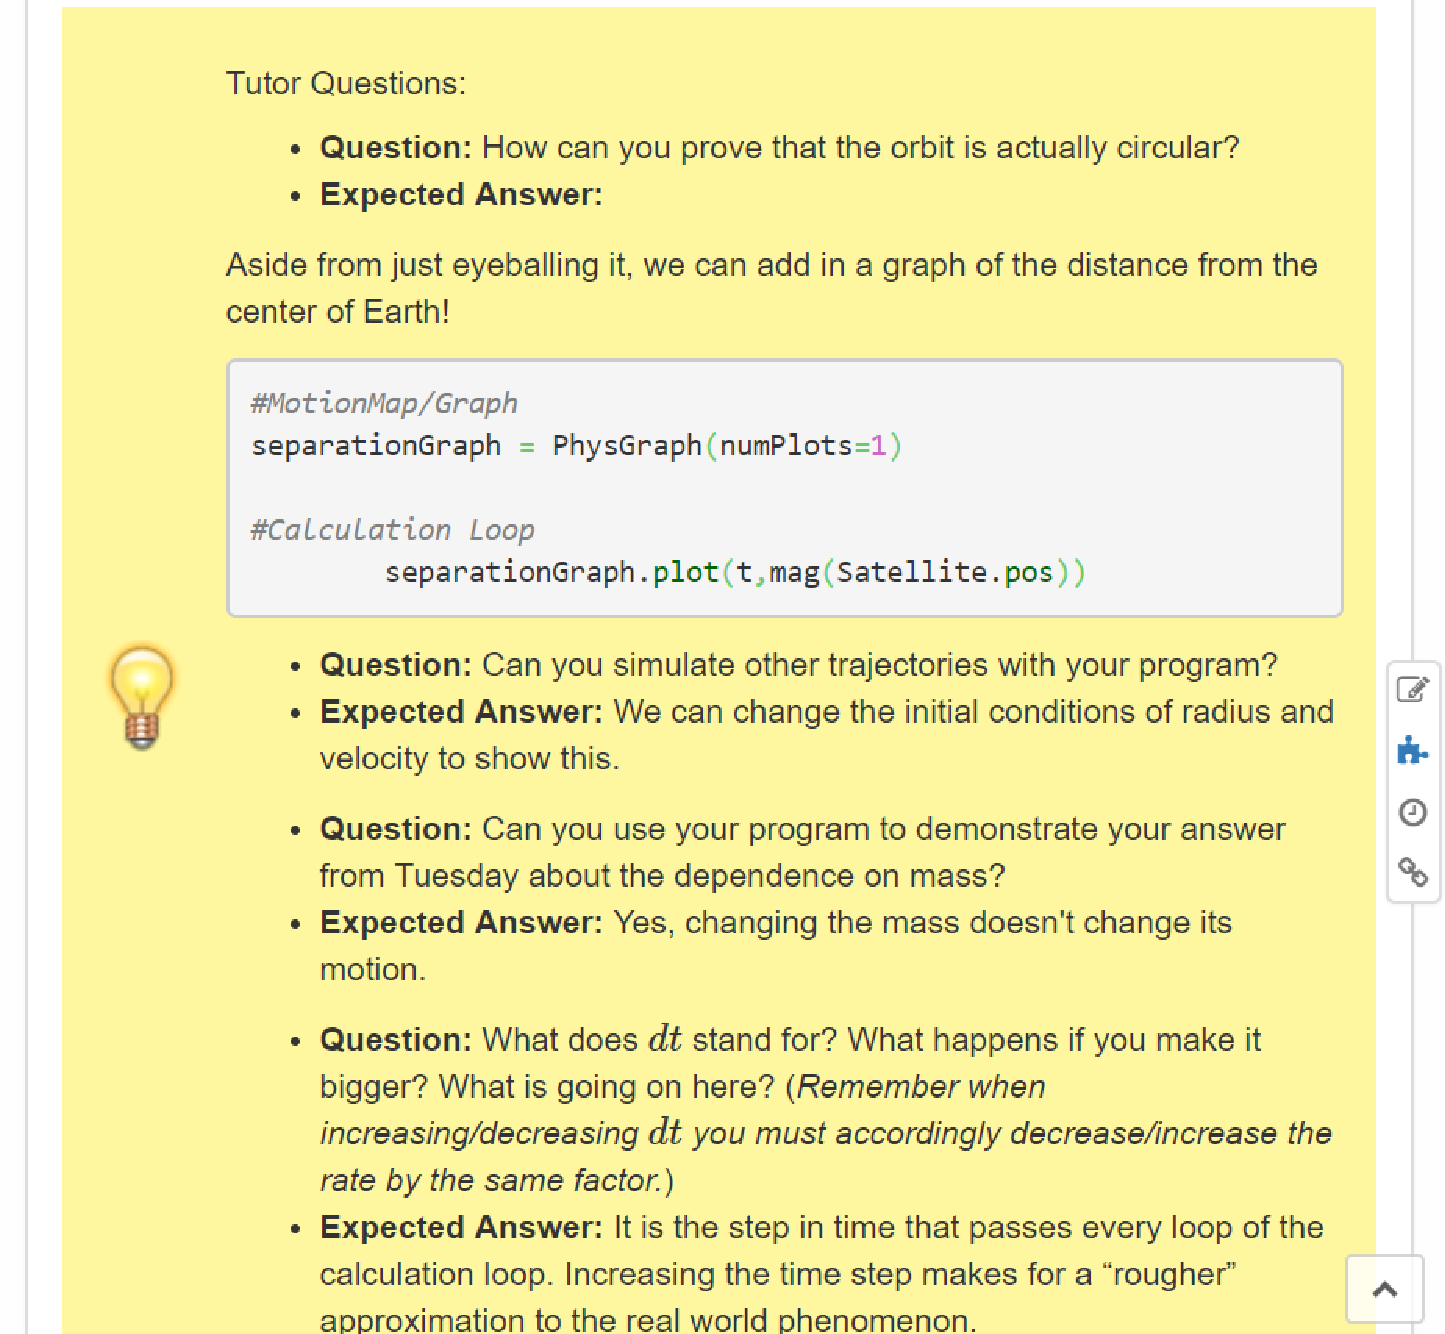
\includegraphics[scale=0.5]{images/CH3TutorQuestion.pdf}
\caption{A seclection of tutor questions that focus on the computational model each group has constructed.}\label{CH3:TutorQuestion}
\end{figure}

On the other hand, a tutor interaction like the one shown below that happens on-the-fly might encourage students to use a more general force rather than a more restricted one:  \begin{description}\TA  you guys wanna talk about what your trategy is at hte moment
\SB  i dont think we know	
\SA we just, we need to figure out how to get the velocity of the spacecraft correct as well as the force net correct and then it should be fine				
\TA yeah, my request, can i point in your program thats what you have for F net now [constant components] my request is to use a completely different strategy where that formula [points to Gmm/r2 on the board] is in for Fnet
\SC yeah we tried to make that yeah		
\SA can we just put the number in?				
\TA umm in principle you could, but id really rather you not have you do it i would like the program to be able to respond if the satellite is father away the force would be less, if the satellite is closer the force would be more so i would like it to be a dynamic program and not one that always have a fixed force\end{description}  In this on-the-fly interaction, the question of weather or not their computational model will be able to handle all types of orbits is enough to indicate that the group needs to switch their model up.  In this way, the tutor is able to make sure the groups stay on the desired path without directly telling them exactly what to do.

\subsection{Feedback/Assessment}

The groups are assessed on many levels in ${\rm P}^{3}$.  One of the most important forms of assessment is given weekly, in the form of written feedback and a numerical score.  The written feedback is based on the observed in-class performance and is designed to point out deficiencies and suggests ways to improve.  The numerical scoring is based on performance in three categories: group understanding, group focus, and individual understanding.

Often the written feedback pertains to group activity with the computer.  For example, the portion of written feedback shown in Fig.~\ref{CH3:WrittenFeedback} is encouraging a student to allow other group members to do some of the typing.   This could be requested for any number of reasons -- most likely, though, because the students with less prior programming experience are not being given a chance to participate.

\begin{figure}[ht]\centering
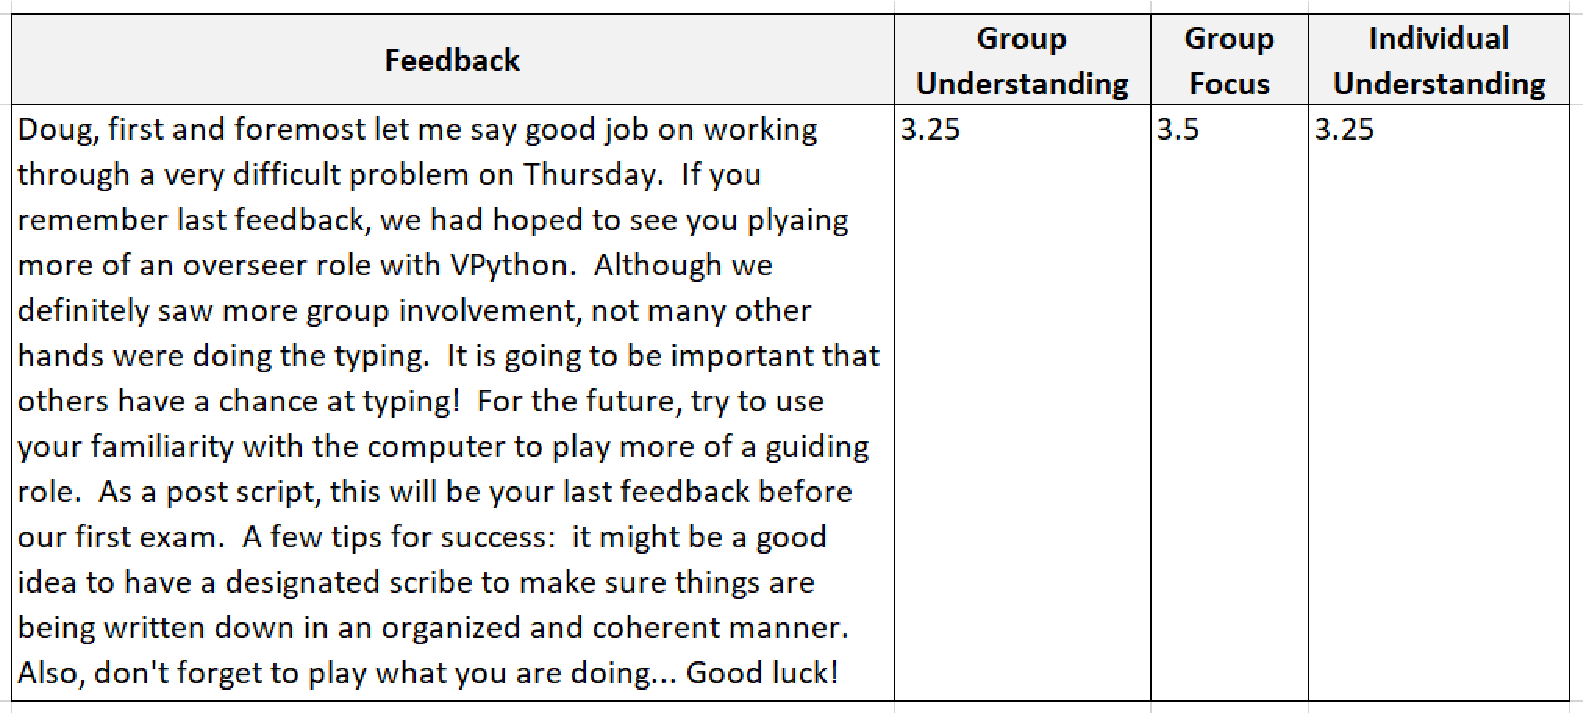
\includegraphics[scale=1.25]{images/CH3WrittenFeedback.pdf}
\caption{A snippet of written feedback given to a student after the third week.}\label{CH3:WrittenFeedback}
\end{figure}

In this way, instructors can encourage their groups to share the programming load.  While doing the typing, it is very difficult to follow along without knowing exactly what is going on.  This helps to engage all of the students with the material.

\section{Post-class work}

There are a number of post-class homework questions that are meant to reinforce the physics and computational concepts seen in class.  During the third week of the course, these questions focus mostly on the Newtonian gravitational force.  However, the post-class homework question shown in Fig.~\ref{CH3:PostClassHomework} that is delivered in the third week focuses on the previous week's computational problem (i.e., it involves a local gravitational force as opposed to a Newtonian gravitational force).  Nevertheless, this post-class question involves the same Euler-Cromer style of numerical integration as seen in all computational problems.  The students are expected to use the error message in order to identify an error in the code.

\begin{figure}[ht]\centering
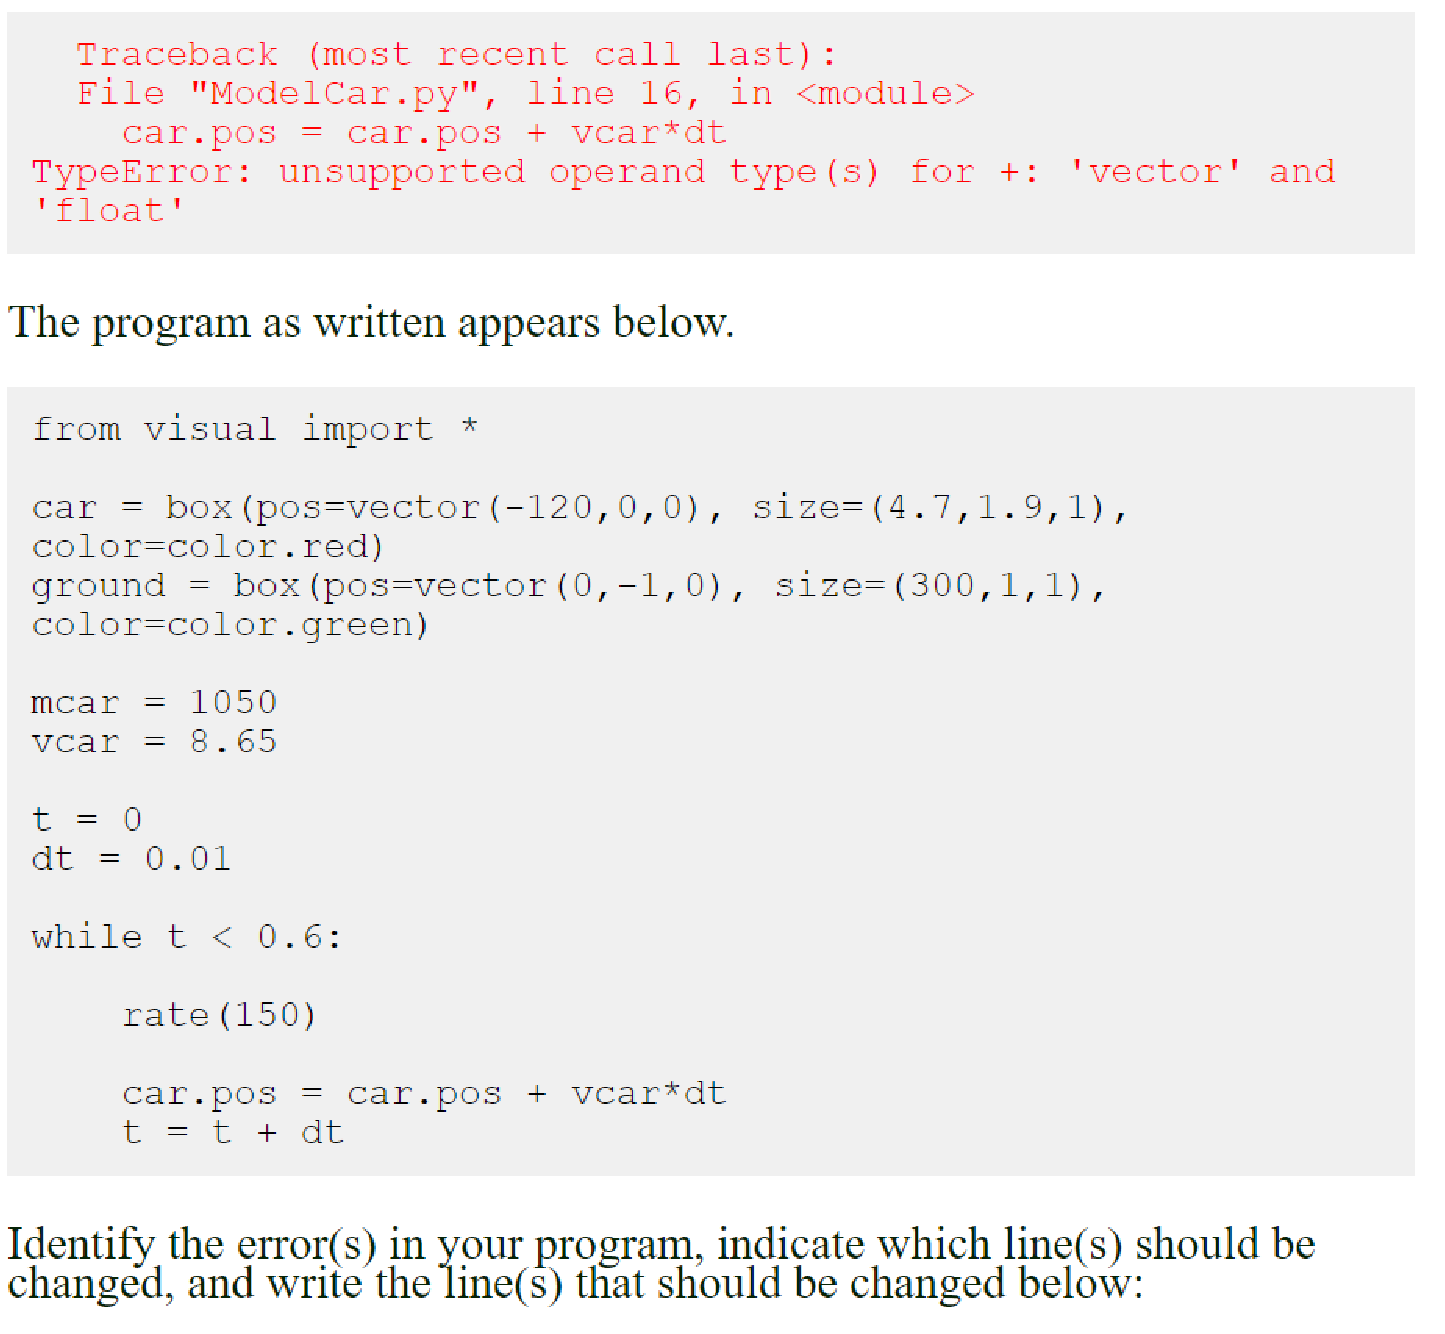
\includegraphics[scale=0.50]{images/CH3PostClassHomework.pdf}
\caption{A portion of a post-class homework question delivered in the third week of the course.  This question requires students to troubleshoot and debug the code.}\label{CH3:PostClassHomework}
\end{figure}

This type of problem helps to encourage students to identify, isolate, reproduce, and correct unexpected problems that arise while constructing computational models.  Ideally, it requires students to interpret the names given to the variables being used and verify that they are defined in a correct form.  Correct form means following one of the basic rules of algebra -- you cannot add a scalar and a vector.

%
%	MOTIVATION
%

\chapter{Motivation}\label{CH4:Motivation}

Aside from a general interest in introductory computational physics, it is important to understand the underlying motivation(s) for this thesis.  The following chapter was published in the proceedings of the 2015 Physics Education Research Conference \cite{AAPT2016}, and is presented here with minor modifications from its appearance in publication. It was published with second and third authors Paul W. Irving and Marcos D. Caballero, respectively.

The process of identifying an interesting computational practice, described in Sec.~\ref{Sec:Debug}, was the earliest motivation for this study.  We found that it was extremely difficult to define and identify the particular practice of what we named ``physics debugging.''  Not only did the practice need to be clearly defined, it also needed to be clearly identified in the data.  This required a lot of in-depth qualitative analysis and inter-rater reliability, motivating our use of the Weintrop framework and the qualitative methods of Clarke et. al.

Additionally, as described in Sec.~\ref{Sec:Phenom}, we found that it was very difficult to understand the qualitatively different ways in which students experienced computational introductory physics.  This difficulty motivated a task analysis with a focus on identifying practices that the students were engaging in through in-class observation, as opposed to their experiences through out-of-class interviews.
  
\section{Debugging}\label{Sec:Debug}

In this section, we present a case study of a group of students immersed in this ${\rm P}^{3}$ environment solving a computational problem.  This problem requires the translation of a number of fundamental physics principles into computer code.  Our analysis consists of qualitative observations in an attempt to describe, rather than generalize, the computational interactions, debugging strategies, and learning opportunities unique to this novel environment.

We focus this case study on the interactions between group and computer to begin to understand the ways in which computation can influence learning.  Particularly, we are interested in the interactions occurring simultaneously with social exchanges of fundamental physics principles (FPPs) specific to the present task (e.g., discussing $d\mathbf{r}=\mathbf{v}\,dt$ on a motion task) and the display of desirable problem solving strategies (e.g., divide-and-conquer).  These group-computer interactions vary in form, from the more active process of sifting through lines of code, to the more passive process of observing a three-dimensional visual display.

One previously defined computational interaction that reinforces desirable strategies, borrowing from computer science education research, is the process of debugging \cite{Fitzgerald2008}.  Computer science defines debugging as a process that comes after testing \emph{syntactically} correct code where programmers ``find out exactly where the error is and how to fix it. \cite{McCauley2008}''  Given the generic nature of the application of computation in computer science environments (e.g., data sorting, poker statistics, or ``Hello, World!'' tasks), we expect to see unique strategies specific to a computational \emph{physics} environment.  Thus, we extend this notion of computer science debugging into a physics context to help uncover the strategies employed while groups of students debug \emph{fundamentally} correct code that produces unexpected physical results.

\subsection{Analysis}

In Fall 2014, ${\rm P}^{3}$ was run at Michigan State University in the Physics Department.  It was this first semester where we collected \emph{in situ} data using three sets of video camera, microphone, and laptop with screencasting software to document three different groups each week.  From the subset of this data containing computational problems, we \emph{purposefully sampled} a particularly interesting group in terms of their computational interactions, as identified by their instructor.  That is, we chose our case study not based on generalizability, but rather on the group's receptive and engaging nature with the project as an \emph{extreme case}.\cite{Flyvbjerg2006}

The project that the selected group worked on for this study consists of creating a computational model to simulate the geosynchronous orbit of a satellite around Earth.  In order to generate a simulation that produced the desired output, the group had to incorporate a position dependent Newtonian gravitational force and the update of momentum, using realistic numerical values.  The appropriate numerical values are Googleable, though instructors encouraged groups to solve for them analytically.

This study focuses on one group in the fourth week of class (the fourth computational problem seen) consisting of four individuals: Students A, B, C, and D.  The group had primary interaction with one assigned instructor.  Broadly, we see a 50/50 split on gender, with one ESL international student.  Student A had the most programming experience out of the group.  It is through the audiovisual and screencast documentation of this group's interaction with each other and with the technology available that we began our analysis.

To focus in on the group's successful physics debugging occurring over the $\SI{2}{\hour}$ class period, we needed to identify phases in time when the group had recognized and resolved a physics bug.  These two phases in time, \emph{bug recognition} and \emph{bug resolution} are the necessary limits on either side of the process of \emph{physics debugging}, as represented in Fig.~\ref{CH4:Phases}.  We identified these two bounding phases at around $\SI{60(5)}{\minute}$ into the problem, and further examined the process of debugging in-between.  That is, we focused on the crucial moments surrounding the final modifications that took the code from producing unexpected output to expected output.

\begin{figure}\centering
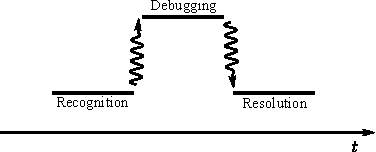
\includegraphics[scale=1]{./images/phases.pdf}
\caption{The debugging process necessarily corresponds to a phase beset on either side by the phases of recognition and resolution.  Note the absence of a vertical scale, as the vertical separation merely acts to distinguish phases.}\label{CH4:Phases}
\end{figure}

\subsubsection{Recognition}

\subsubsection{Resolution}

\section{Phenomenography}\label{Sec:Phenom}

A description of the phenomenography study.

\subsection{Protocol}

A description of the development of the protocol.

\subsection{Analysis}

Since there are no real results, we can just describe how we analyzed the interview data.

%
%	ANALYSIS
%

\chapter{Analysis}\label{CH5:Analysis}

\section{Specific methods}

Following the suggestion of thematic analysis, we begin with a full transcription of the in-class video.  This transcription is verbatim to the best of our abilities.  Any inaudible sections are indicated, with long pauses being indicated by ellipses ($\ldots$).  To distingish between unspoken actions (e.g., pointing to an equation) and infereces made by the researcher (e.g., refering to a previous equation), we follow the convention of square brackets ($[\,]$) and curly brackets ($\{\,\}$), respectively.

This full transcript is then read through multiple times, noting any points of interest in terms of the Weintrop framework.  We then divide the transcript into multiple excerpts of shorter length centered around the initial points of interest.  Although we lose some of the coherence of the problem as a whole by focusing on shorter exerpts, these relatively shorter exerpts help to facilitate a deeper analysis.  Each transcript contains $\approx\SI{1500}{lines}$ comprising $\approx\SI{50}{excerpts}$.

Each excerpt is analyzed in terms of the practices the group is engaging in.  This means we need to look for the characteristics of each practice. With these characteristics identified, we are justified in classifying the particular excerpt as that practice.  Each excerpt generally has between one and four identified computational practices. 

Each characteristic that is identified is supported with rationale on three levels: the rationale according to the framework, the rationale within the excerpt, and the rationale beyond the excerpt.  The confidence in this rationale (specifically, the rationale within the excerpt) manifests itself in a high, medium, and low confidence rating for the identification of this practice.  In that way, we know not only how frequently the practices are identified, but also how confident we are in that assessment.

\begin{figure}[ht]\centering
%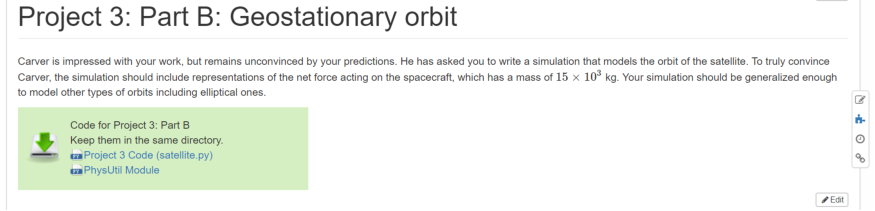
\includegraphics[scale=1]{images/CH3SatelliteProblem.pdf}
\caption{Visual representation of the different levels of rationale pertaining to an excerpt.  Green, yellow, and red cells represent high, medium, and low confidence, respectively.}\label{CH3:VariableAnalysis}
\end{figure}

We indicated confidence by marking a potentially identified practice as either high (green), medium (yellow), or low (red) confidence.  To determine confidence, however, a process of inter-rater reliability was conducted between three raters.  This process included sharing a representative sample of the excerpts and converging on the actual practices observed.  Rationale for every high- to medium-confidence practice, then, is provided according to the framework, according to the data within the excerpt, and according to any data beyond the excerpt.

With these practices identified, we then analyzed their frequency.  Many practices showed up frequently, and some showed up almost never.  These simple statistics, like $${\rm frequency\,of\,particular\,practice}=\frac{\rm number\,of\,particular\,practice\,observed}{\rm number\,of\,all\,practices\,observed},$$ give us a concrete way to hone in and focus our analysis on the most important (or at least frequent) practices.

The most important practices were then further analyzed for the variation in the characteristics that make up each practice.

So that we safeguard against the researcher influencing the results too much, inter-rater reliability is checked at multiple points throughout the analysis.  This check consists of an independent researcher (the inter-rater) identifying practices with confidence in a reduced set of the data and comparing with the primary researcher.  Any practices in which confidence is questioned and lost are discounted from being identified.

\section{Findings}

Recall that, according to the framework, each category of practice can be broken down into a number of individual practices.  Each individual practice, further, can be identified in terms of a number of fundamental characteristics.  Depending on the particular situation, some categories show up in the data more often than others.  For example, we expect to see fewer systems thinking practices and more computational modeling practices.  Further, within any category, some individual practices show up in the data more than others.  For example, within the data practices, we expect to see fewer instances of collecting data and more instances of creating data.

Most importantly, within any individual practice, there is a broad set of defining characteristics.  Ideally, each characteristic would be present in some form when its corresponding practice has been identified.  However, each characteristic can be organized in terms of being either necessary or sufficient for the cause.  That is, we need not necessarily observe every characteristic in order to identify a practice according to the framework.

\begin{figure}[ht]\centering
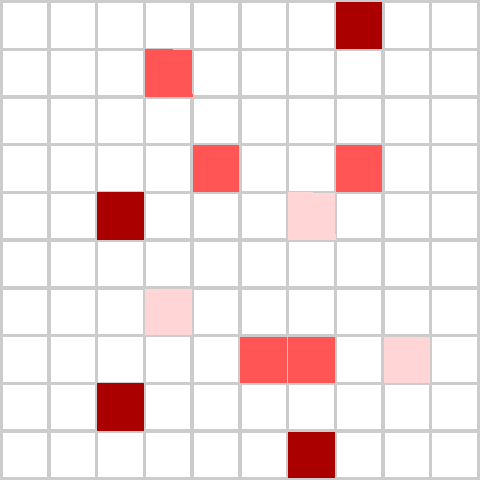
\includegraphics[scale=1]{./images/matrix.pdf}
\caption{A ``density plot'' for all computational practices and all groups.}\label{CH5:DensityPlot}
\end{figure}

\subsection{Assessing computational models}

The most important computational modeling practice indicative of computational thinking is that of assessing computational models.  This practice shows up $\SI{100}{\percent}$ of the time.  Assessing computational models seems to be crucial to the process of designing and constructing computational models.  Given that computational models take a lot of work and iteration to get to an acceptable level, it is no surprise that assessing shows up so frequently.

There are three characteristics that are necessary to be observed in an excerpt to warrant classification of ``assessing computational models.''  The first characteristic that needs to be observed is a ``model.''  There are several models that show up in the data.  The second characteristic that needs to be observed is a ``phenomenon.''  For the most part, the phenomena are related to the simulation of the trajectory of the geostationary satellite and its various physical interpretations (e.g., a central attractive force or a circular orbit).  The third characteristic that needs to be observed is a ``comparion'' between the model and phenomenon.  The comparisons that we see are ultimately varied, given that they depend on not only the model but also the phenomenon.

\begin{figure}[ht]\centering
\begin{tabular}{l|c|r}
a & b & c \\\hline
c & d & $\SI{100}{\percent}$ \\
\end{tabular}
\caption{A table showing rough statistics for assessing computational models.}\label{CH5:AssessingComputationalModels}
\end{figure}

\subsubsection{Computational model}

The two big models that we have observed in the data are a position dependent Newtonian gravitational force in terms of a separation vector and a centripetal force that depends on the polar angle of the satellite.  Each model shows up $\SI{100}{\percent}$ and $\SI{100}{\percent}$ of the time, respectively.

\subsubsection{Phenomenon}

The phenomena that we have observed in the data are almost always centered around the simulation of the trajectory of the satellite.  The physical interpretations of the phenomena are, not surprisingly, closely related to the topics covered in the couse notes and the topics questioned in the weekly homework.  These interpretations range from the crude (e.g., a circular orbit) to the sophisticated (e.g. a centripetal force and its properties).  This variety of phenomena show up $\SI{100}{\percent}$ of the time.

\subsubsection{Comparison between}

The comparisons that we have observed in the data are quite varied.  Given that the comparison is between the models and phenomena, we expect this characteristic to be the most varied.

\subsection{Creating data}

\subsubsection{Data set}

\subsubsection{Algorithmic procedure}

\subsubsection{Advance understanding}

%
%	DISCUSSION
%

\chapter{Discussion}\label{CH6:Discussion}


\section{Primary practices}

Analyzing data, assessing computational models, programming, and thinking in levels are the most common practices that we observed.

\section{Secondary practices}

Creating data, constructing computational models, creating computational abstractions, and understanding the realations within a system are the lesser common practices that we observed.

\section{Absent practices}

Some of the practices that were not observed in the data were collecting data and choosing effective computational tools.

%
%	CONCLUSIONS
%

\chapter{Conclusion}\label{CH7:Conclusion}

The most important things that you should be paying attention to are the creation and analysis of data, the assessment and construction of models, programming and troubleshooting, and thinking in levels and communicating

%
%	APPENDICES
%

\appendices

\chapter{Additional excerpts}

%
%	BIBLIOGRAPHY
%

\end{doublespace}

\bibliography{bibliography}
\bibliographystyle{plain}

\end{document}

%
%	EXTRA
%

\begin{landscape}
\thispagestyle{empty}
\captionof{table}{caption_text}
\captionof{figure}{caption_text}
\end{landscape}

\begin{figure}
\center
\begin{enumerate}
\item Data
\begin{enumerate}
\item Collecting
\begin{enumerate}
\item Propose protocols
\item Articulate automation
\end{enumerate}
\item Creation
\begin{enumerate}
\item Define procedures
\item Run simulations
\item Create data
\item Advance understanding
\end{enumerate}
\item Analysis
\item Visualization
\end{enumerate}
\item Modeling and Simulation
\item Problem Solving
\item Systems Thinking
\end{enumerate}
\caption{The framework developed by Weintrop et. al to describe the computational practices observed in science and mathematics classrooms.  Each category contains between five and seven individual practices, and each practice has between two and seven fundamental characteristics.}\label{CH2:Framework}
\end{figure}